\documentclass[11pt, a4paper]{article}
\usepackage[english, science, small]{ku-frontpage}
\usepackage[utf8]{inputenc}
\usepackage[cache=false]{minted}
\usepackage{caption}
\usepackage{subcaption}
\usepackage[linesnumbered,ruled]{algorithm2e}
\usepackage{algpseudocode}
\usepackage{gensymb}

% Math stuff
\usepackage{amsmath,amssymb,mathtools,bm,etoolbox,stmaryrd}
% verctor command. Usage: \colvec{5}{a}{b}{c}{d}{e}
\newcount\colveccount
\newcommand*\colvec[1]{
	\global\colveccount#1
	\begin{pmatrix}
		\colvecnext
	}
	\def\colvecnext#1{
		#1
		\global\advance\colveccount-1
		\ifnum\colveccount>0
		\\
		\expandafter\colvecnext
		\else
	\end{pmatrix}
	\fi
}

% que dymbol, textmode
\newcommand*{\qed}{\hfill\ensuremath{\square}}%

% TOC properties
\setlength\arraycolsep{2 pt}
\setcounter{tocdepth}{2}
\setcounter{secnumdepth}{2}

\author{Per Steffen Czolbe (wjq874) \& Asger Hans Skovbjerg Christensen (tzw174)}
\title{Reinforcement Learning with LEGO Mindstorms}
\subtitle{Project Report}
\date{Handed in: \today}

\begin{document}
\maketitle

\section{Abstract}

\tableofcontents


\section{Introduction}
Machine learning growing in interest, and is getting wildly popular. Google trends show an almost 4 times increase in searches for "machine learning" over the last 5 years\cite{googletrendsML}, and many online sites and universities are offering courses on it.

The term "Machine Learning" refers to a collection of algorithmic and statistical models, as well as related data handling methods, and deals with many classical statistical problems, such as regression and classification, using more automated model approaches, relying on computers and algorithms for optimization and model improvement.

This increasing interest in machine learning can serve as a foundation for earlier introduction to related topics, such as "overfitting", "training" and more generally "data". This could satisfy or feed the growing popularity, as well as generate more interest in and funding for university level and industry machine learning. 

An industry that's currently looking into machine learning is LEGO. Among other things, LEGO develops educational aids, to inspire children of different age groups and create an interest in STEM (Science, Technology, Engineering and Maths)\cite{LEGOeducation}. LEGO both sells educational aids and collaborates directly with schools\cite{naerheden}. This project exists partially because LEGO contacted DIKU about machine learning, specifically interests in reinforcement learning. They were inspired by videos, in which people had used reinforcement learning with their LEGO Mindstorms robots to teach them to perform actions by learning on their own\cite{youtube_crawl}\cite{youtube_swing}. Reinforcement learning is a subject of machine learning that concerns itself with which action an actor should take to optimize reward on a future scale, and usually involves gathering data by trying actions and observing the consequences. 

LEGO was interested in the methods, to see how easily this could be implemented and how large the space of potential educational use was.

This additional interest allows us to implement machine learning and reinforcement learning methods in practice, studying the practical implications when learning data is gathered in the physical world. It also means that we're interested in exploring the complexity and width of the space of educational use of LEGO Mindstorms for explaining and teaching machine learning and reinforcement learning. Thus, we intend to built robots and implement reinforcement learning algorithms on them, or create visualizations of training and prediction of models using them, to explore the complexity of this task, as well as the width of the subject both for future studies and for educational use. Each robot will be designed with a goal in mind, to learn some task and possibly visualize it, and as much as possible, they will cover a wide variety of methods. The code for the project is written in Python through Jupyter notebooks, and can be found on GitHub\footnote{https://github.com/SteffenCzolbe/LEGO-machine-learning}.

\section{EV3 System}
The EV3 system is the third version of the LEGO Mindstorm family of robot toys. It contains a central processing component, called ''Brick``, to which motors, sensors and other peripheral devices can be attached. All components are embedded into plastic casings, which make them compatible with other LEGO parts. The LEGO Group markets the EV3 system to educational facilities and private persons in a package with build instructions and parts for multiple robots. The current product offering consists of 2 different packages to build a total of 9 robots, including the self-balancing two wheeled ``Gyroboy'' and a sorting machine that orders LEGO bricks based on their colour. The playful development of further robots by end users is encouraged. A large community of engaged hobby robot builders has formed around the EV3 platform.

This section examines the components, motors, sensors and software of the EV3 ecosystem. We combine these components later on to build our own robots.

\subsection{Central component: The Brick}
The Brick is the central processing component of each EV3 robot. It can be controlled via multiple buttons, features a small LCD screen and can be connected to a computer via Wifi, Bluetooth or USB. For peripherals, up to 4 motors and 4 Sensors can be connected. The specifications of the embedded system are \cite{ev3_dev_toolkit}:
\begin{listing}
	CPU: 32bit, 300MHz ARM9 Processor \\
	Memory: 64Mb DDR RAM\\
	Storage: 16Mb Flash, up to 32Gb SD-Card \\
	Communication: USB, Bluetooth, Wifi \\
	Peripherals: 4 motors, 4 Sensors
\end{listing}

\subsection{Motors}
The LEGO product line includes a variety of 9V DC electrical motors, which can be used to power a wide range of LEGO models, such as cars, trains and robots. The current product offering consists of two main families: ``Power Functions'' motors and ``EV3'' servo motors. The most common sizes of these product lines are shown in figure \ref{fig:motors}.

\begin{figure}
	\centering
	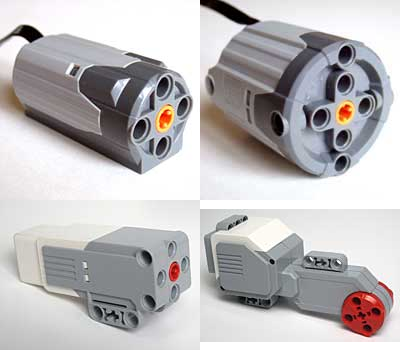
\includegraphics[width=0.4\linewidth]{images/motors}
	\caption{Overview of current (2018) LEGO motors. Upper row: Power Functions large and X-large motor. Bottom row: EV3 medium and large motor. Images from \cite{motor_comparison}.}
	\label{fig:motors}
\end{figure}

\subsubsection*{Power Functions Motors}
The ``Power Functions'' line of motors is designed to work with a battery pack and is intended to be controlled either with a physical switch on the battery pack or a remote control. Adapters for the power cables are required to use them in combination with the EV3 platform. \cite{power_fun}

By changing the current and polarity of the DC power supply, these motors can spin in both directions and different speeds. Because `Power Functions'' motors do not measure rotation or angle, robots utilizing them often require other means of measuring mechanical movements. Compared to the EV3 servo motors, they offer similar torque and mechanical power, have faster reaction speeds but offer no feedback. \cite{motor_comparison}


\subsubsection*{EV3 Servo Motors}
The EV3 robot kit contains a medium and two large servo motors. The EV3 motors use tacho feedback to measure their alignment and rotation, which allows for more precise control compared to ``Power Functions'' motors. \cite{Servo_Motor}. In strength and speed they are comparable to their ``Power Functions'' counterparts. The large EV3 motor is roughly twice as powerful as the medium one, and comes in a bigger case with different mounting points. Detailed comparisons of the mechanical and electrical properties of all LEGO motors is available at \cite{motor_comparison}.

The ev3dev programming environment offers functions for low level interactions with the EV3 motors. Available are methods to start and stop the motor, reading the angle, setting the speed and three different stopping patterns (coast, brake and hold). The medium and large EV3 Motor offer identical programming interfaces. For angle measurements, the motor saves the rotation at system start as 0 degrees. During operation, the current rotation angle offset to the starting point can be read by the motor. \cite{ev3_python}

\subsection{Sensors}
While motors make the robot move, sensors are used to observe the environment and deliver a base for making decisions. In this section we provide an overview over button, colour sensor, ultrasonic sensor and gyroscope.

\subsubsection*{Button}
One of the simplest sensors of the EV3 system is the button. It is a box-shaped sensor, where one side has a spring loaded retractable surface. This surface is the button. The sensor has two states: pushed and not pushed. Buttons are often used as an event triggers, were a push of the button starts a programmed action.




\subsubsection*{Colour Sensor}
The EV3 colour sensor works by shining red, green, blue or all three colours of light and measuring values of the reflections. The sensor can measure colours, ambient light and reflected light. When retrieving colours, the sensor cycles all three LEDS rapidly, when retrieving reflected light, only the red led is on, and when retrieving ambient light, only the blue led is on\cite{colour_sensor_python}. The colour sensor has a built-in list of possible colours, and can measure and predict white, blue, black, green, red, yellow, brown and no colour. Since the sensor measures reflection, pointing it into the air will measure (close to) (0,0,0) which it categorises as no colour.

\subsubsection*{Ultrasonic Sensor}
The EV3 Ultrasonic Sensor generates sound waves and reads their echoes to detect and measure distance from objects. It can also send single sound waves to work as sonar or listen for a sound wave that triggers the start of a program. Distances mesured range from 0-250cm. While the python bindings of this sensor return a distance measurement with an accuracy of up to 1mm \cite{ev3_python}, LEGO advertises an accuracy of  ``up to +/-1cm''. \cite{ultraosnic_sensor}

While working with the sensor on the crawling robot, we noticed the importance of mounting the sensor on a stable frame. It should not tilt vertically or horizontally, as any change in angles also changes the distance to a target. To attain accurate and reliable distance measurements, the target should be a rather large, solid plane, oriented orthogonal to the ultrasonic waves emitted by the sensor. The accuracy is sufficient to measure sub-centimetre movements. Roughly 0.1\% of measurements were faulty and reported the maximum distance value of 255cm. No further experiments to evaluate the accuracy of the ultrasonic sensor have been performed.

\begin{figure}[H]
	\centering
	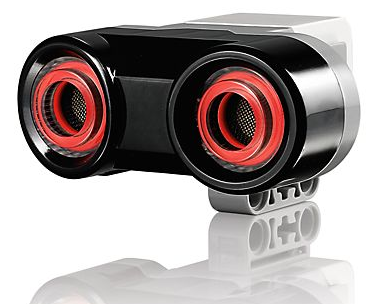
\includegraphics[width=0.3\linewidth]{images/ultrasonic}
	\caption{The EV3 ultrasonic sensor. Image from \cite{ultraosnic_sensor}.}
	\label{fig:ultrasonic}
\end{figure}

\subsubsection*{Gyroscope}
The gyroscope sensor detects rotational motion in the plane. This can be used to measure motion of a robot. Applications are self-balancing robots, or measuring the angle of a turn of a driving robot.

The gyroscope sensor is an accelerometer. It measures angular acceleration with a sample rate of 1kHz. By taking the integral of the acceleration, it is able to approximate angles \cite{gyroscope}. Since the gyroscope relies on calibration and its angle measurements are an approximation, they are often highly unreliable. We discuss ways of dealing with this in the calibration and accuracy section.


\subsection{Software}
The EV3 platform is sold with a software system centred around LEGO's own proprietary graphical programming language based on LabVIEW. The programming language with a graphical interface enables people with limited programming experience to quickly develop simple programs that can be executed on the Brick. The graphical language is supported by an editor available as a program for Windows and Mac, and as an app for Android and iOS.

While the default software is well supported by the editor and operating system of the brick, more experienced programmers might prefer a more capable language. Multiple community driven software packages exist for this purpose. These support languages such as matlab, python, java, javascript, C++, C, GO, Ruby, Perl, R, Lua, even direct control of the robot via command line is possible \cite{ev3dev}. We discuss a specific development set up in the next section.



\section{Development Setup}
In this section we present the development set up chosen for this project. It consists of the open source operating system ev3dev to power the brick, the ev3dev python library to control motors and sensors, and remote procedure calls to communicate with the robot from a host computer the via jupyter notebook.

\subsection{Ev3dev Platform}
Ev3dev is a Debian Linux-based operating system that runs on several LEGO Mindstorms compatible platforms including the LEGO Mindstorms EV3 and Raspberry Pi-powered BrickPi. It is maintained by a community of enthusiasts and offers libraries to interact with LEGO Mindstorms motors and sensors in many programming languages, such as Java, Ruby and Python \cite{ev3dev}. The Linux disk image can be downloaded at \href{https://www.ev3dev.org/}{www.ev3dev.org} and flashed on a SD card. Once the SD card is inserted into the LEGO Mindstorms brick, the brick will boot into the ev3dev operating system. A set up guide with detailed explanations on installation and guides on how to get started with development are available at the ev3dev website.

\subsection{Control by external Computer}
While the brick, after flashed with the ev3dev image, runs a Debian Linux system that can execute general purpose programs, the processing and memory constraints imposed by the hardware limit the complexity of programs executed on the brick severely. Installing a python package takes 2 minutes. Executing more computationally expensive tasks like deep learning or real time video processing on the brick is not feasible.

To circumvent these problems, a setup of the main program running on a computer and interacting with the brick to move motors or read sensor data has been employed by multiple community projects, such as a rubics cube solver \cite{ev3_rubics}. We follow the design approach pioneered by these projects. The brick runs a remote procedure call server, implemented by the python3 library \texttt{rpyc}. This allows a host computer to connect to the brick and remotely interact with motors and sensors. All program logic is executed on the computer, the brick is listening to commands. Next to the performance improvements, another benefit is that the program can be executed in a jupyter notebook on the computer, which allows to better integrate documentation and visualization into the development process.

\section{Accuracy and Calibration}
To build models that can demonstrate reinforcement learning reliably, we need accurate and reproducible sensor measurements and motor movements. We design experiments to measure the time delay and accuracy of sensors and motors. We empirically determine which ways of controlling the motors yields the most reliable outcomes, and discuss which sensors need to be calibrated before use. 
\subsection{Time Delays}

We tested the response time of the motors, buttons and the colour sensor, to get an understanding of how quickly we would be able to react, as well as how reliable this connection was. \footnote{The code for this can be found commented in experiments/Response speed experiment.ipynb.} 

For the button, a single button was connected, and we measured the time until the robot noticed that the button wasn't pressed, and repeated, this setup was very simple and was repeated 1000 times taking 19s. Mean button response was $0,019$s with a very low variance at $4,8\cdot 10^{-6}$s$^2$.

Motor reaction speed was tested with a slightly more complicated setup, in which a large motor had an arm attached, that had to move to hit a button. The arm was positioned right in front of the button, such that any amount of movement would set off the button, and it would reset position after each round. A video of this setup can be found in the notebook. Motor response testing was repeated 1000 times, and took 85s. Since the time involved a button delay, a value without this was calculated by substracting the button delay mean. The mean of the new motor-only delay was $0,066$ seconds and the motor had much higher variance than the button at $3,6\cdot 10^{-4}$ seconds$^2$ and a $95\%$ percentile of $0,124$ seconds. This is also clearly visible in Figure \ref{fig:responsetimemotorbutt}.

\begin{figure}[H]
	\centering
	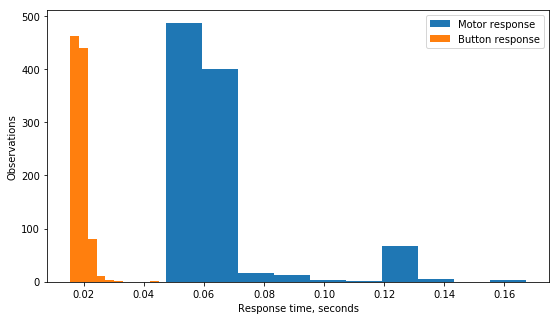
\includegraphics[scale=0.7]{images/motor_button_response_histogram.png}	
	\caption{Histogram of  response times from buttons and motors.}
	\label{fig:responsetimemotorbutt}
\end{figure} 
From this it appears that motor response is not only slower, but also a bit more unstable than the button response. Note though, that more factors, such as speed and real-world interference could have affected the motor response speed experiment. Still, even if assuming the 95\% percentile, we should be able to get at least 8 actions per second.

The colour sensor turned out to react significantly slower than the button, probably due to the fact that it has to cycle between different LEDs. An experiment was made in which a colour sensor made an RGB observation and this time was logged. It was compared to an experiment in which it observed both RGB, reflected light and ambient light. Both were run 10.000 times, taking 10 and 38 minutes respectively.

\begin{figure}[H]
	\centering
	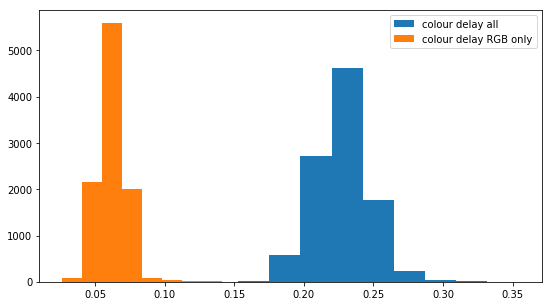
\includegraphics[scale=0.7]{images/colour_response_histogram.png} 	
	\caption{Histogram of  response times from the colour sensor if requesting only RGB colours, and if ambient and reflected light is also requested.}
	\label{fig:responsetimecolour}
\end{figure}
With only RGB, we observed a mean response time of $0,062$ seconds, which is very comparable to the motor response time, but with a lower variance at $1,1\cdot 10^{-4}$. With everything, the mean response was $0,228$ seconds and a variance of $3,8 \cdot 10^{-4}$. The distribution of these response times can be seen in Figure \ref{fig:responsetimecolour}, from which it seems that the response times are at least low variance.

It might be possible to reduce the delay by storing information on the brick such that the transfer between brick and computer only happens once, but since the connection delay is at most $0,012$s (as evident from the button delay), the delay would still be significantly longer than RGB only.


\subsection{Motor Accuracy}
Reinforcement learning algorithms rely on repetition of the same motions many times. To assume a non-adversarial environment and ensure reproducible results, actions taken by the motors need to be accurate and consistent. We design an experiment to measure the accuracy of the motors after a series of repeated actions.

\subsubsection*{Experimental Setup}
The experiment consists of an arm attached to a motor. We rotate the arm in a 90 degree angle back and forth. After every 25 iterations we measure the offset from the starting position externally with a set square. To measure the influence of weight on the results we use two independent arms, one without a weight and the other one weighted by three heavy metals balls. The experimental set-up is shown in figure \ref{fig:angle_experiment}.

\begin{figure}[H]
\centering
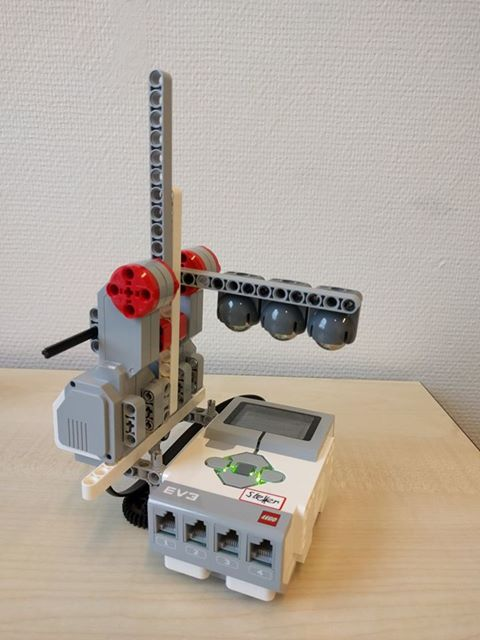
\includegraphics[width=0.35\linewidth]{images/angle_experiment}
\caption{Experiment to measure motor accuracy. The two arms (gray) swing back and forth in a 90 degree angle. One arm is weighted down by three heavy metal balls.}
\label{fig:angle_experiment}
\end{figure}



The ev3dev python bindings offer two different movement patterns: \texttt{'on\_for\_degrees()'}, which rotates the motor relative to the current position, and \texttt{'move\_to\_pos()'}, which rotates the motors to an absolute value.  Further, three stopping patterns exists: \texttt{'brake'}, \texttt{'hold'} and \texttt{'coast'}. In the experiment we will test different combinations of movement and holding patterns, to determine the configuration with the highest amount of accuracy and reproducibility. Since we want high accuracy, we do not test the \texttt{'coast'} setting. The coasting option allows the motors to 'coast' until standstill, instead of enforcing them to stop at a specific position. 


\begin{table}[H]
	\centering
	\begin{tabular}{|l|l|l|l|l|l|l|}
		\hline
		Move Pattern & Stop Pattern & Weight & inaccuracy after 25 iterations & after 50it & after 75it             & after 100it            \\ \hline \hline
		relative   & hold         & no     & 1\degree             & 1\degree    & 2\degree                & 2\degree                \\ \hline
		relative   & hold         & yes    & 9\degree             & 11\degree   & 35\degree               & 45\degree               \\ \hline
		relative   & brake        & no     & 1\degree             & 1\degree    & 1\degree                & 2\degree                \\ \hline
		relative   & brake        & yes    & 35\degree            & 50\degree   & \textgreater{}50\degree & \textgreater{}50\degree \\ \hline
		absolute     & hold         & no     & 0\degree             & 1\degree    & 2\degree                & 1\degree                \\ \hline
		absolute     & hold         & yes    & 2\degree             & 1\degree    & 4\degree                & 3\degree                \\ \hline
		absolute     & brake        & no     & 1\degree             & 2\degree    & 2\degree                & 3\degree                \\ \hline
		absolute     & brake        & yes    & 4\degree             & 6\degree    & 5\degree                & 4\degree                \\ \hline
	\end{tabular}
	\caption{Experimental result. Angle offset in degrees after 25, 50, 75 and 100 iterations for different configurations.}
	\label{tab:angle_experiment}
\end{table}


\subsubsection*{Results}
The angle offsets measured after 25, 50, 75 and 100 iterations for different motor control settings and configurations are shown in table \ref{fig:angle_experiment}. As we can see, the non-weighted arm is very accurate in all scenarios. The results for the weighted arm differ drastically between configurations. We can observe two trends:
\begin{enumerate}
	\item The \texttt{'brake'} stopping pattern creates more offset than the \texttt{'hold'} pattern. Further observations of the experiment let us conclude that \texttt{'brake'} stops the motion of the motor, but does not block the motor for further movement after the initial momentum has been eliminated. This leads to the weighted arm pulling slightly further down between the breaking phase and the next swing of the arm. The \texttt{'hold'} stop motion holds the arm in place even after the initial momentum is eliminated. It leads to more accurate results under load.
	\item Movements ot absolute positions are more precise than relative movements. While inaccuracies of relative movements accumulate over time, movements to absolute positions only carry the inaccuracy of the last movement.
\end{enumerate}
During the experiment we also measured the range of motion that is possible without receiving any push-back from the motors. This amount of slack is consistently measured at about 12 degrees. No configuration lowered this inaccuracy. If it causes a problem later on, mechanical solutions such as a worm gear could be used to reduce the slack.

\bigskip
In conclusion, to attain the highest level of accuracy and reproducibility, motors should be moved to absolute positions and the stop pattern \texttt{'hold'} should be used. We note however that motors still allow for free movement of about 12 degrees without providing any breaking or pushback.

\subsection{Gyroscope Accuracy}
A common complain about the EV3 system is the unreliability of the gyroscope sensor. Users commonly report issues with a 'drift' of measurements, where a non-moving sensor reports a constant non-zero speed, and angle measurements that shift over time \cite{gyro_inaccurate}. It appears that without any extra steps, the gyroscope sensor is the most unreliable out of all sensors available for the EV3 platform.

To understand the drift in angle measurements, we have to understand how the gyroscope works. Even though the sensor is marketed as a gyroscope, it is an accelerometer. The sensor measures acceleration. Based on the acceleration measurements, it calculates the first integral to approximate speed, and the second integral to approximate a position or angle. When initializing, the sensor assumes to be standing still. Thus the acceleration level measured at system start is assumed to be no acceleration. If there is a slight inaccuracy, the speed and angle approximations accumulate errors over time. To reduce the drift, it is important to calibrate the sensor very accurately, for example by ensuring there is no motion in the system when it is powered on. However, the drift can not be eliminated completely. Even highly accurate gyroscopes, as used for example in space exploration, experience a drift an angle measurements by about 1 degree a year. In consumer goods, the drift is more significant, with mobile phones commonly experiencing drift of over 1 degree a minute \cite{gyro_drift}. To account for this drift, it is important to re-calibrate the sensor frequently.

Once the sensor is properly calibrated, it measures \texttt{angle} and \texttt{rate}, where \texttt{rate} describes the rate of angle change in degrees per second. Figure \ref{fig:pendulum} visualizes values obtained from the sensor. In the experiment we attach the gyroscope to a pendulum of $30$cm length and raise the pendulum to an angle of approx 60 degrees. We release the pendulum and plot measurements taken during the swinging motion. We can observe that the angle, plotted in blue, forms a declining sinus form, as the pendulum swings back and forth. In orange we see the acceleration, which by manual inspection seems to be roughly the first derivative of the angle measurements, as we would expect.

\begin{figure}
\centering
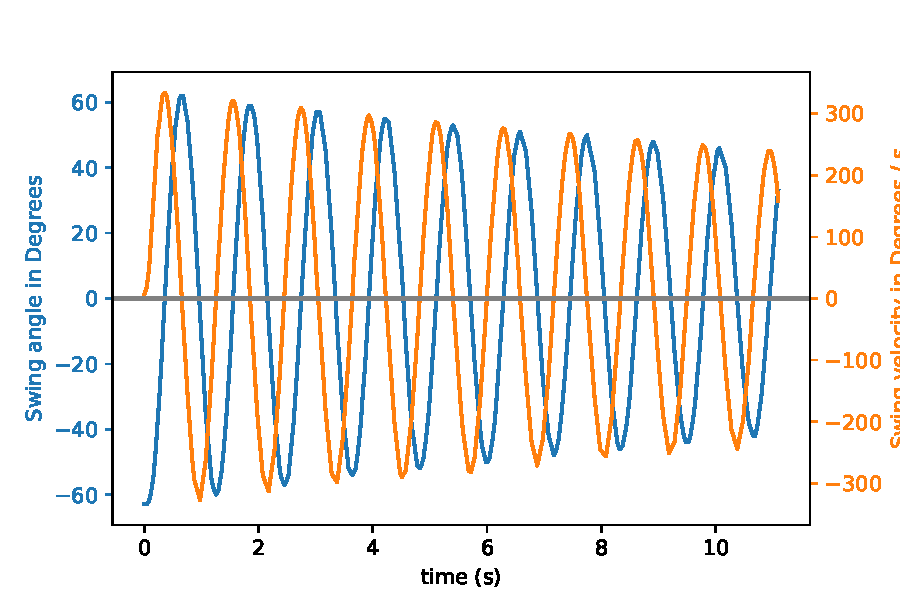
\includegraphics[width=0.6\linewidth]{images/pendulum}
\caption{Measurement of a well calibrated gyroscope attached to a pendulum. Angle of the pendulum in blue, acceleration in orange. No drift in angle measurements is apparent in the 10 second timeframe.}
\label{fig:pendulum}
\end{figure}


\subsection{Calibration} \label{calibration}
Servo motors and gyroscope sensors are initialized when the brick is restarted, the colour sensor has a built-in white value which can be recalibrated. All other sensors require no calibration.

On system start, the position of the motor is initialized as 0 degrees. If the robot is dependent on absolute positional values, it is important to calibrate the 0-point. This can either be done by moving the motor forcefully into the correct position before starting the brick, or using more elaborate constructions of moving the motor against a button, until the button is pressed. This gives certainty over the 0-position of the motor and can be used to calibrate the rotation.

The gyroscope initializes its orientation at system start as 0 degrees. Further, it assumes to be not in motion during system start. All acceleration measurements are in relation to this value taken during system start. Since the rotational angle returned by the gyroscope is calculated as the integral over acceleration measurements, even a slight inaccuracy in acceleration will accumulate to a significant drift in angle over time. This drift has to be monitored and adjusted for. This can be done either programmatic, or by restarting the system to re-calibrate the sensor.

The colour sensor can be re-calibrated to a new relative white, but this is only used for normalization of observed colour values (originally from 0-1020) to the RGB scale. If not recalibrated, the sensor uses 300 as the maximal expected white value.

\pagebreak
\section{Colour Detection}
\subsection{Problem}
A common first topic when learning about machine learning is the KNN algorithm, as it's simple to understand, allowing it to be a comparison for other models, or a base model to use when explaining other topics not specific to a model.

The colour sensor was chosen as a way to visualize KNN. We wanted to be able to visualize how machine learning updated after data was added and what the basis for decisions were, using a simple and easy to understand setup, expanding on the simplicity of KNN by adding visual or even physical aids.
\subsection{Robot Design}
The robot was built to be easy to use and consistent to allow similar observations from the colour sensor at different times.

A mount was made for the sensor, that easily plugged into the robot, and which could provide readings from everything placed on top of it, allowing for regular distances to the observed object at one regular LEGO Technic block. Two buttons where added to the side of the robot for controls.

The final design is simple and modular, allowing it to be easily disassembled into smaller parts and reassembled later, and can be seen in Figure \ref{fig:colour_robot_full_shot}.\footnote{More pictures found in additional\_robot\_images/Colour\_robot}

\begin{figure}[H]
	\centering
	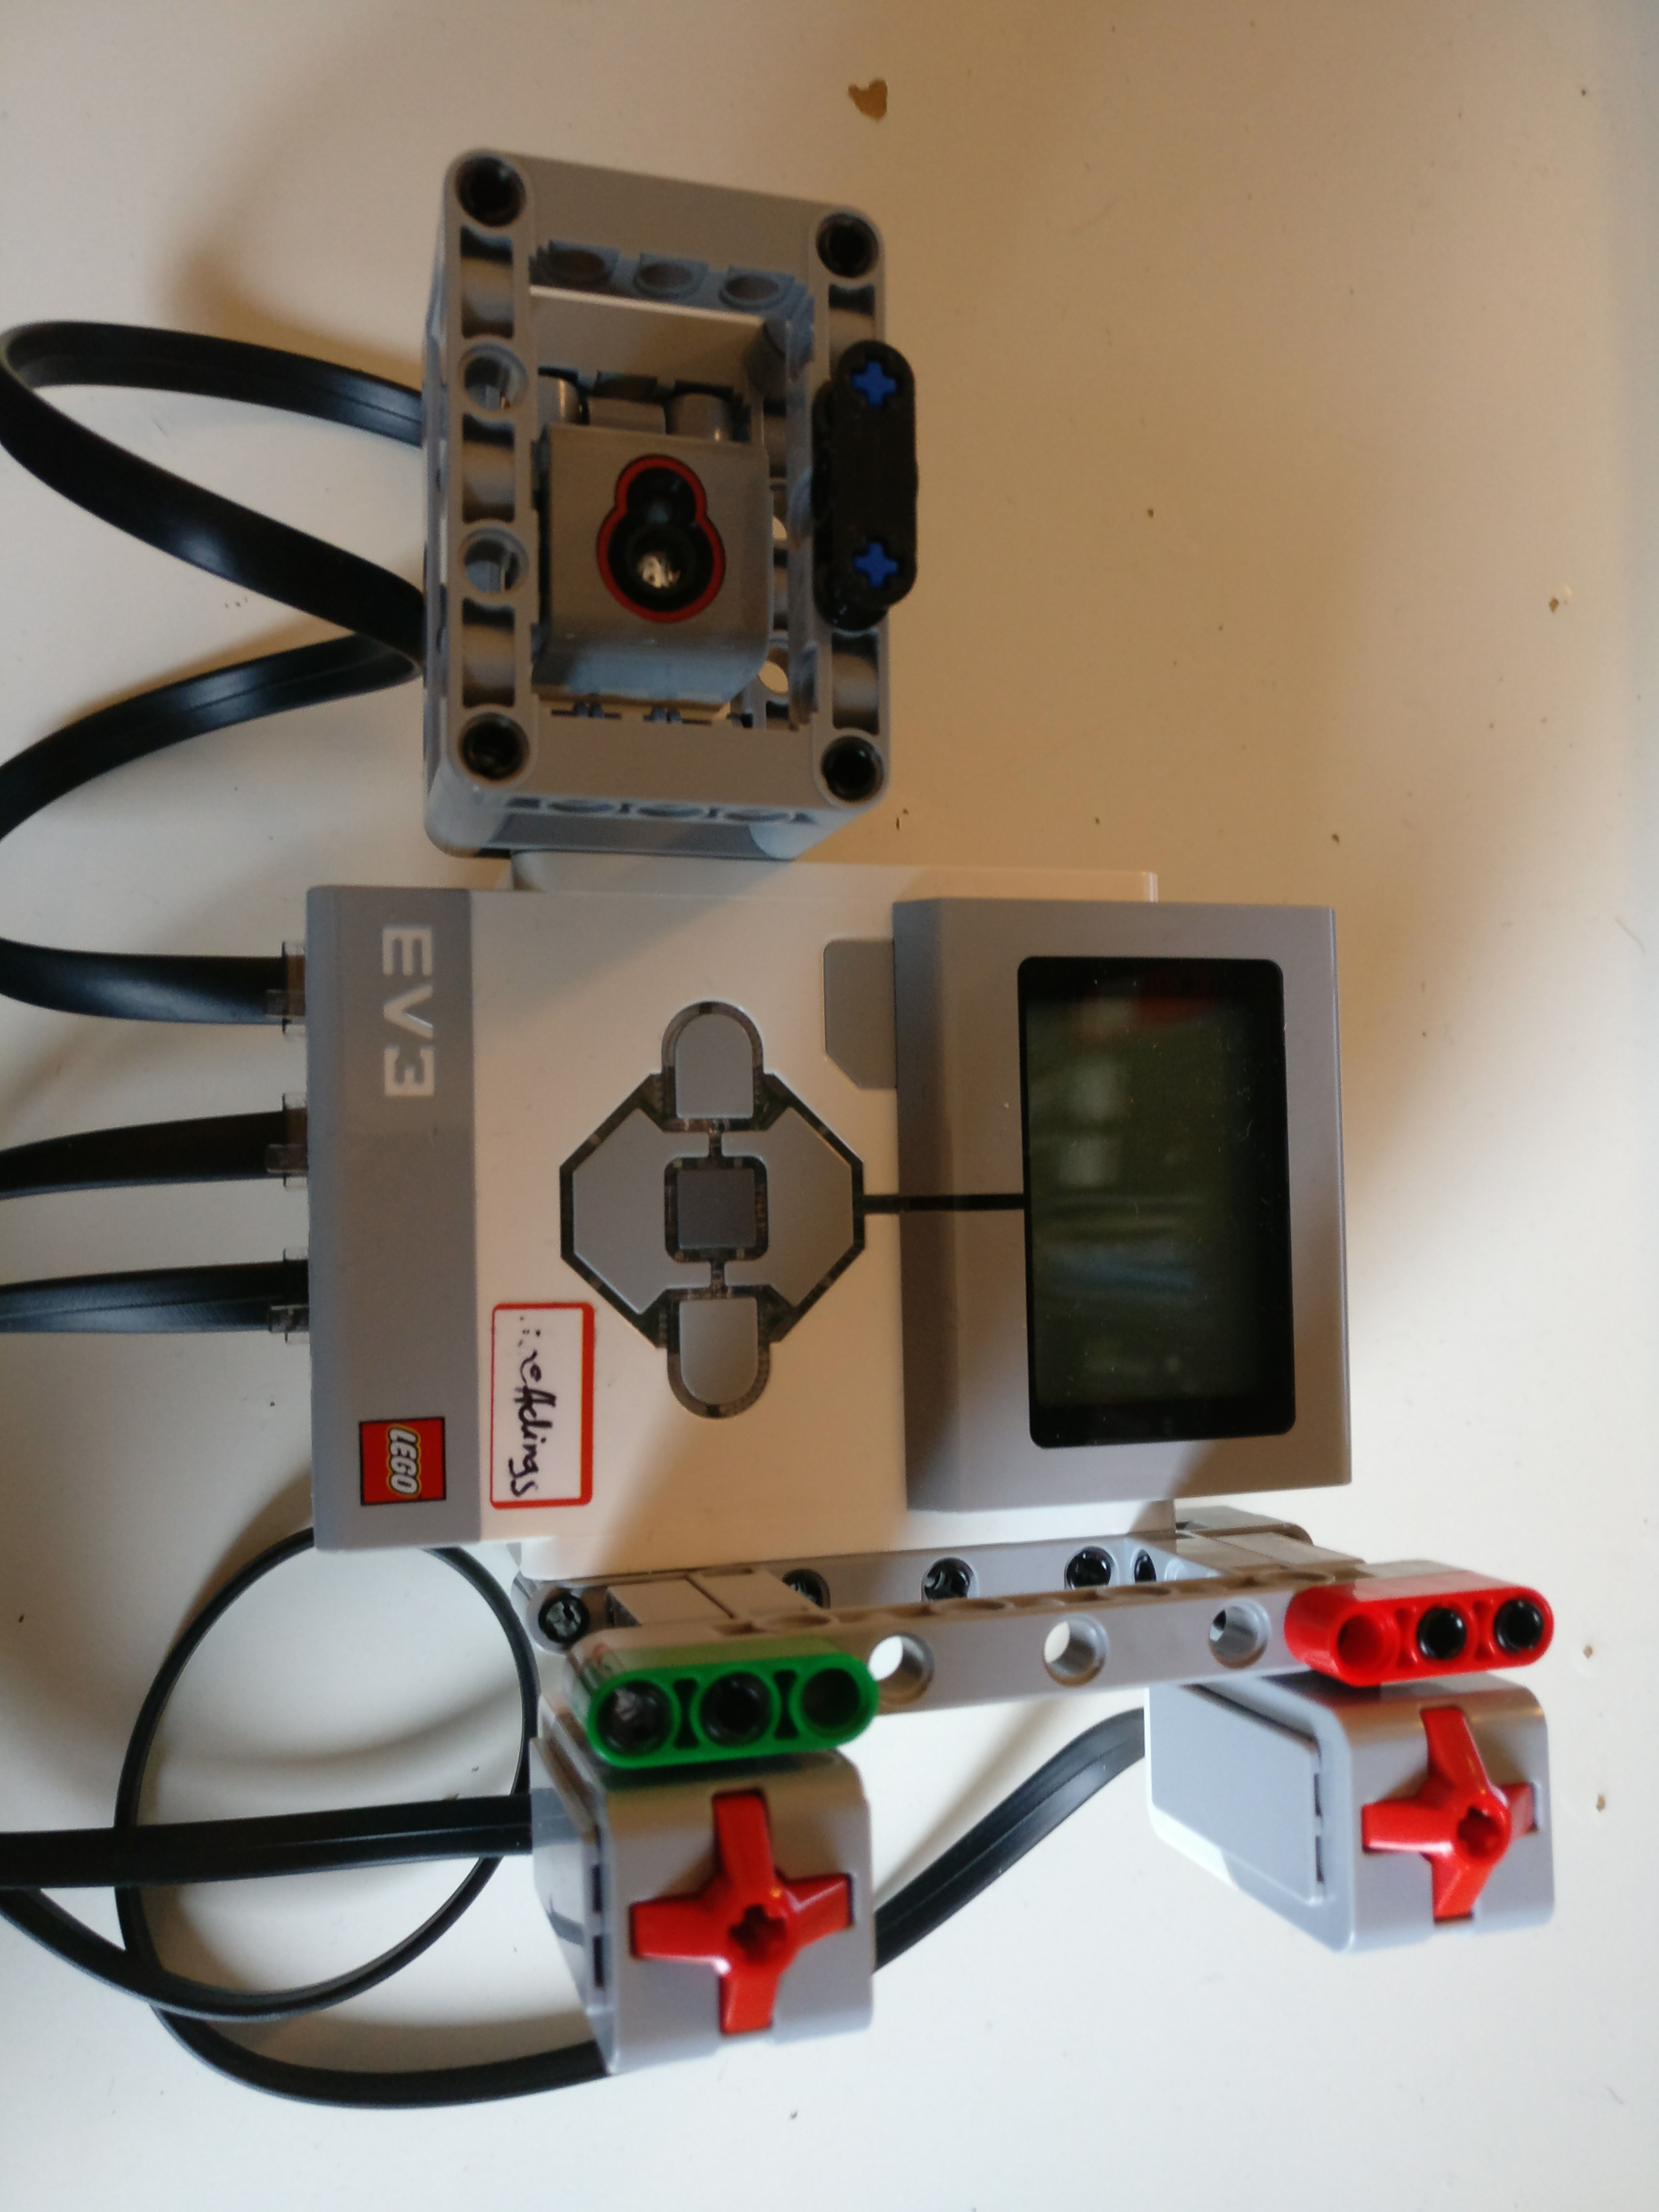
\includegraphics[scale=0.05,angle=90]{images/colour_robot_full.jpg} 	
	\caption{Full top shot of the colour robot, featuring the colour sensor and mount (left side), the brick (middle) and the buttons (right side).}
	\label{fig:colour_robot_full_shot}
\end{figure}
Since the robot has no moving parts, the results should be easily replicateable as along as the robot is built with 2 buttons and a color sensor, and the matter is kept still at a distance of one block.
\subsection{The Learning}
As planned we implemented KNN, as one of the simplest and most intuitive machine learning algorithms. For the data input we used only the RGB output from the color sensor. We wanted to plot in real time, and learned from the time-experiments that calling more values proved too much of a delay. For visualization, we used a 3d-plot of the observed colors, with the axes being red, green and blue values.

We made two versions of KNN with the color sensor\footnote{The code for both of these is found commented in simple\_learning/KNN colors.ipynb}, and a more advanced neural network model\footnote{The code for this is commented in reinforcement\_colors/reinforced\_colors.ipynb.}
\subsubsection{Colour learning: Internal LEGO based model}
The first version is slightly silly, but colorful. Our dataset is started with either a base set (simple RGB values) or a few observations, in which we use the color sensor's built in predictions. Real-time KNN is then run, and we output our prediction as well as a 3d plot of our current observation (black triangle), together with all previous observations (coloured dots). Additional dots can be added by pressing a button, which adds the current observation and prediction as a true point in the data. This produces colourful plots, as seen in Figure \ref{fig:colour_KNN_LEGO}.

\begin{figure}[H]
	\centering
	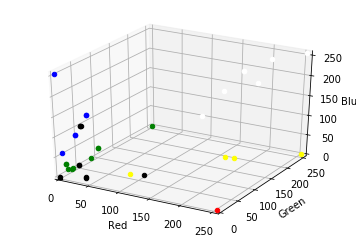
\includegraphics[scale=1]{images/ColourKNNversion1.png} 	
	\caption{Visualization output from the LEGO based KNN model. Here each coloured dot represents a data point with corresponding RGB values and the represented colour. Current observation, represented by a black square, is not featured.}
	\label{fig:colour_KNN_LEGO}
\end{figure}
\subsubsection{Colour learning: Binary classifier}
Since the above version uses starting data and the built-in predictions from LEGO, we also tried a different setup. Instead of prediction colours directly, we predict colour groups, which we will call group "red" and group "green". In this setup, the robot again predicts and plots in real time, but we now start with zero data, and rely only on the buttons. One button adds the prediction to the data set with label "red" and the other "green". This allows us to not rely on anything from LEGO, and allows us to make different splits, such as light versus dark colours, which could learn to differentiate light and dark blue. The plots are similar to before, but with fewer colours, as seen in figure \ref{fig:colour_KNN_binary}.

\begin{figure}[H]
	\centering
	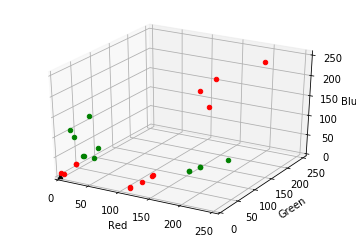
\includegraphics[scale=1]{images/ColourKNNversion2.png}	
	\caption{Visualization output from the binary KNN model. Here each coloured dot represents a data point with corresponding RGB values and the represented group. Current observation, represented by a black square, is seen in the bottom left, near (0,0,0).}
	\label{fig:colour_KNN_binary}
\end{figure}
\subsubsection{Colour learning: Neural Network and subject width}
Finally, we implemented a more complicated system to work with other visualizations. We implemented a neural network, and wanted to visualize how learning and training works in this setup. 

In this case, the robot has a list of allowed colors, starts with no data, and predicts from an untrained network. It reads RGB colours, but also reflected light and ambient light, since we are not running real-time. It displays scores for each color, and reads the highest scoring color aloud. A button press indicates whether this was correct or wrong, and it trains based on this feedback. This allows the user to view updates in predictions from step to step. The predictions are output on a list like below, updated with every new prediction \\

'Black : 0.13146167' \\

'Blue : 0.20897976' \\

'Green : 0.15094219' \\

'Red : 0.22930987' \\

'White : 0.14744666' \\

'Yellow : 0.13185982' 

\subsection{Sub-results}
Two versions of a robot that uses KNN were implemented and built with visualization in mind. Both versions are functional, and can be used to explain and link how data affects predictions in machine learning.

We implemented a simple Neural Network model, that may be useful in explaining more complicated machine learning models.

We also learned a great deal about visualization and limitations to this, which will be presented and discussed in the following section.
\subsection{Discussion}
We encountered a number of difficulties related to these experiments, but have also found many avenues of possible future work.
\subsubsection{Discussion: Visualization}
We originally wanted to show the decision boundary for our learning system, to show how it changes with time. Unfortunately, we found no good way to visualize this in 3d, so instead we looked into dimensionality reduction. We tried reducing dimensionality using PCA, and plot a decision boundary in the resulting 2d space, but this proved problematic, both in our setup and generally. Since we wanted to run real-time we had issues running the PCA on the decision boundary. To get enough points for a proper boundary in 3d space we had to use at least 1 million points, which took way too long to process to be able to run real-time. If instead we didn't run real-time, we could plot the PCA values and a decision boundary in this space, but the values would be mostly meaningless. In the 3d space it at least somewhat makes sense, you have an intuition about what changes if we increase on the "red" axis and so on. In the PCA space we're left with principal components instead, and the points from previous observations would not even be stationary.

Some ways to get around this issue would be to only read two colour channels (removing the need to reduce dimensionality), or find another experiment which only takes two inputs. 
\subsubsection{Discussion: Neural Network and future work}
The neural network setup was made to demonstrate that the colour sensor setup can be extended to more complicated machine learning systems, to show some width of the space of possible educational use. It was implemented, but as a very simple form. It takes a number of colours initially, and predicts between these, but for more than 2 colours (or colour groups) this makes training complicated. The model was implemented such that if it predicted the first colour on our list, and we respond correct, it trains with (1,0,0,0) (or similar for more colours) while instead if we respond wrong, it trains (0,1,1,1) (so it improves every other colour). This setup is not optimal, and is simply a POC. If instead we want to focus on this task to improve it, it may be able to use methods from reinforcement or online learning, since we're dealing with a reduced feedback (right/wrong) setup (this was an idea from the start, as is obvious from the file name). The reason this wasn't implemented was a time constraint built into the setup. At the moment, prediction is done by pressing both buttons, which causes the prediction list to update, and the robot to say the highest scoring colour. At this point you can press a button for yes or no. Unfortunately, you need a lot of observations to properly train the network, which makes it very time consuming and not very education-friendly. We ran a test with 150 entries, observing only 3 different colours. After this, it could still not differentiate the 3 colours. We believe that implementing a proper reinforcement or bandit setup would greatly improve the training, but 150 observations or just 50 that all have to be done manually is still a significant barrier for the neural network setup. Other options could be to pre-load it with some amount of data, but this would remove the chance to see early learning. The output for the neural network model could of course be combined with a plot like the 3d we made for the KNN model, or a PCA/decision boundary or similar, with most of the same yields and issues as discussed before. We believe the neural network setup has potential, but has some hurdles to overcome before it can be useful in an educational setting.

\pagebreak
\section{Crawl-Robot}
\begin{figure}[H]
	\centering
	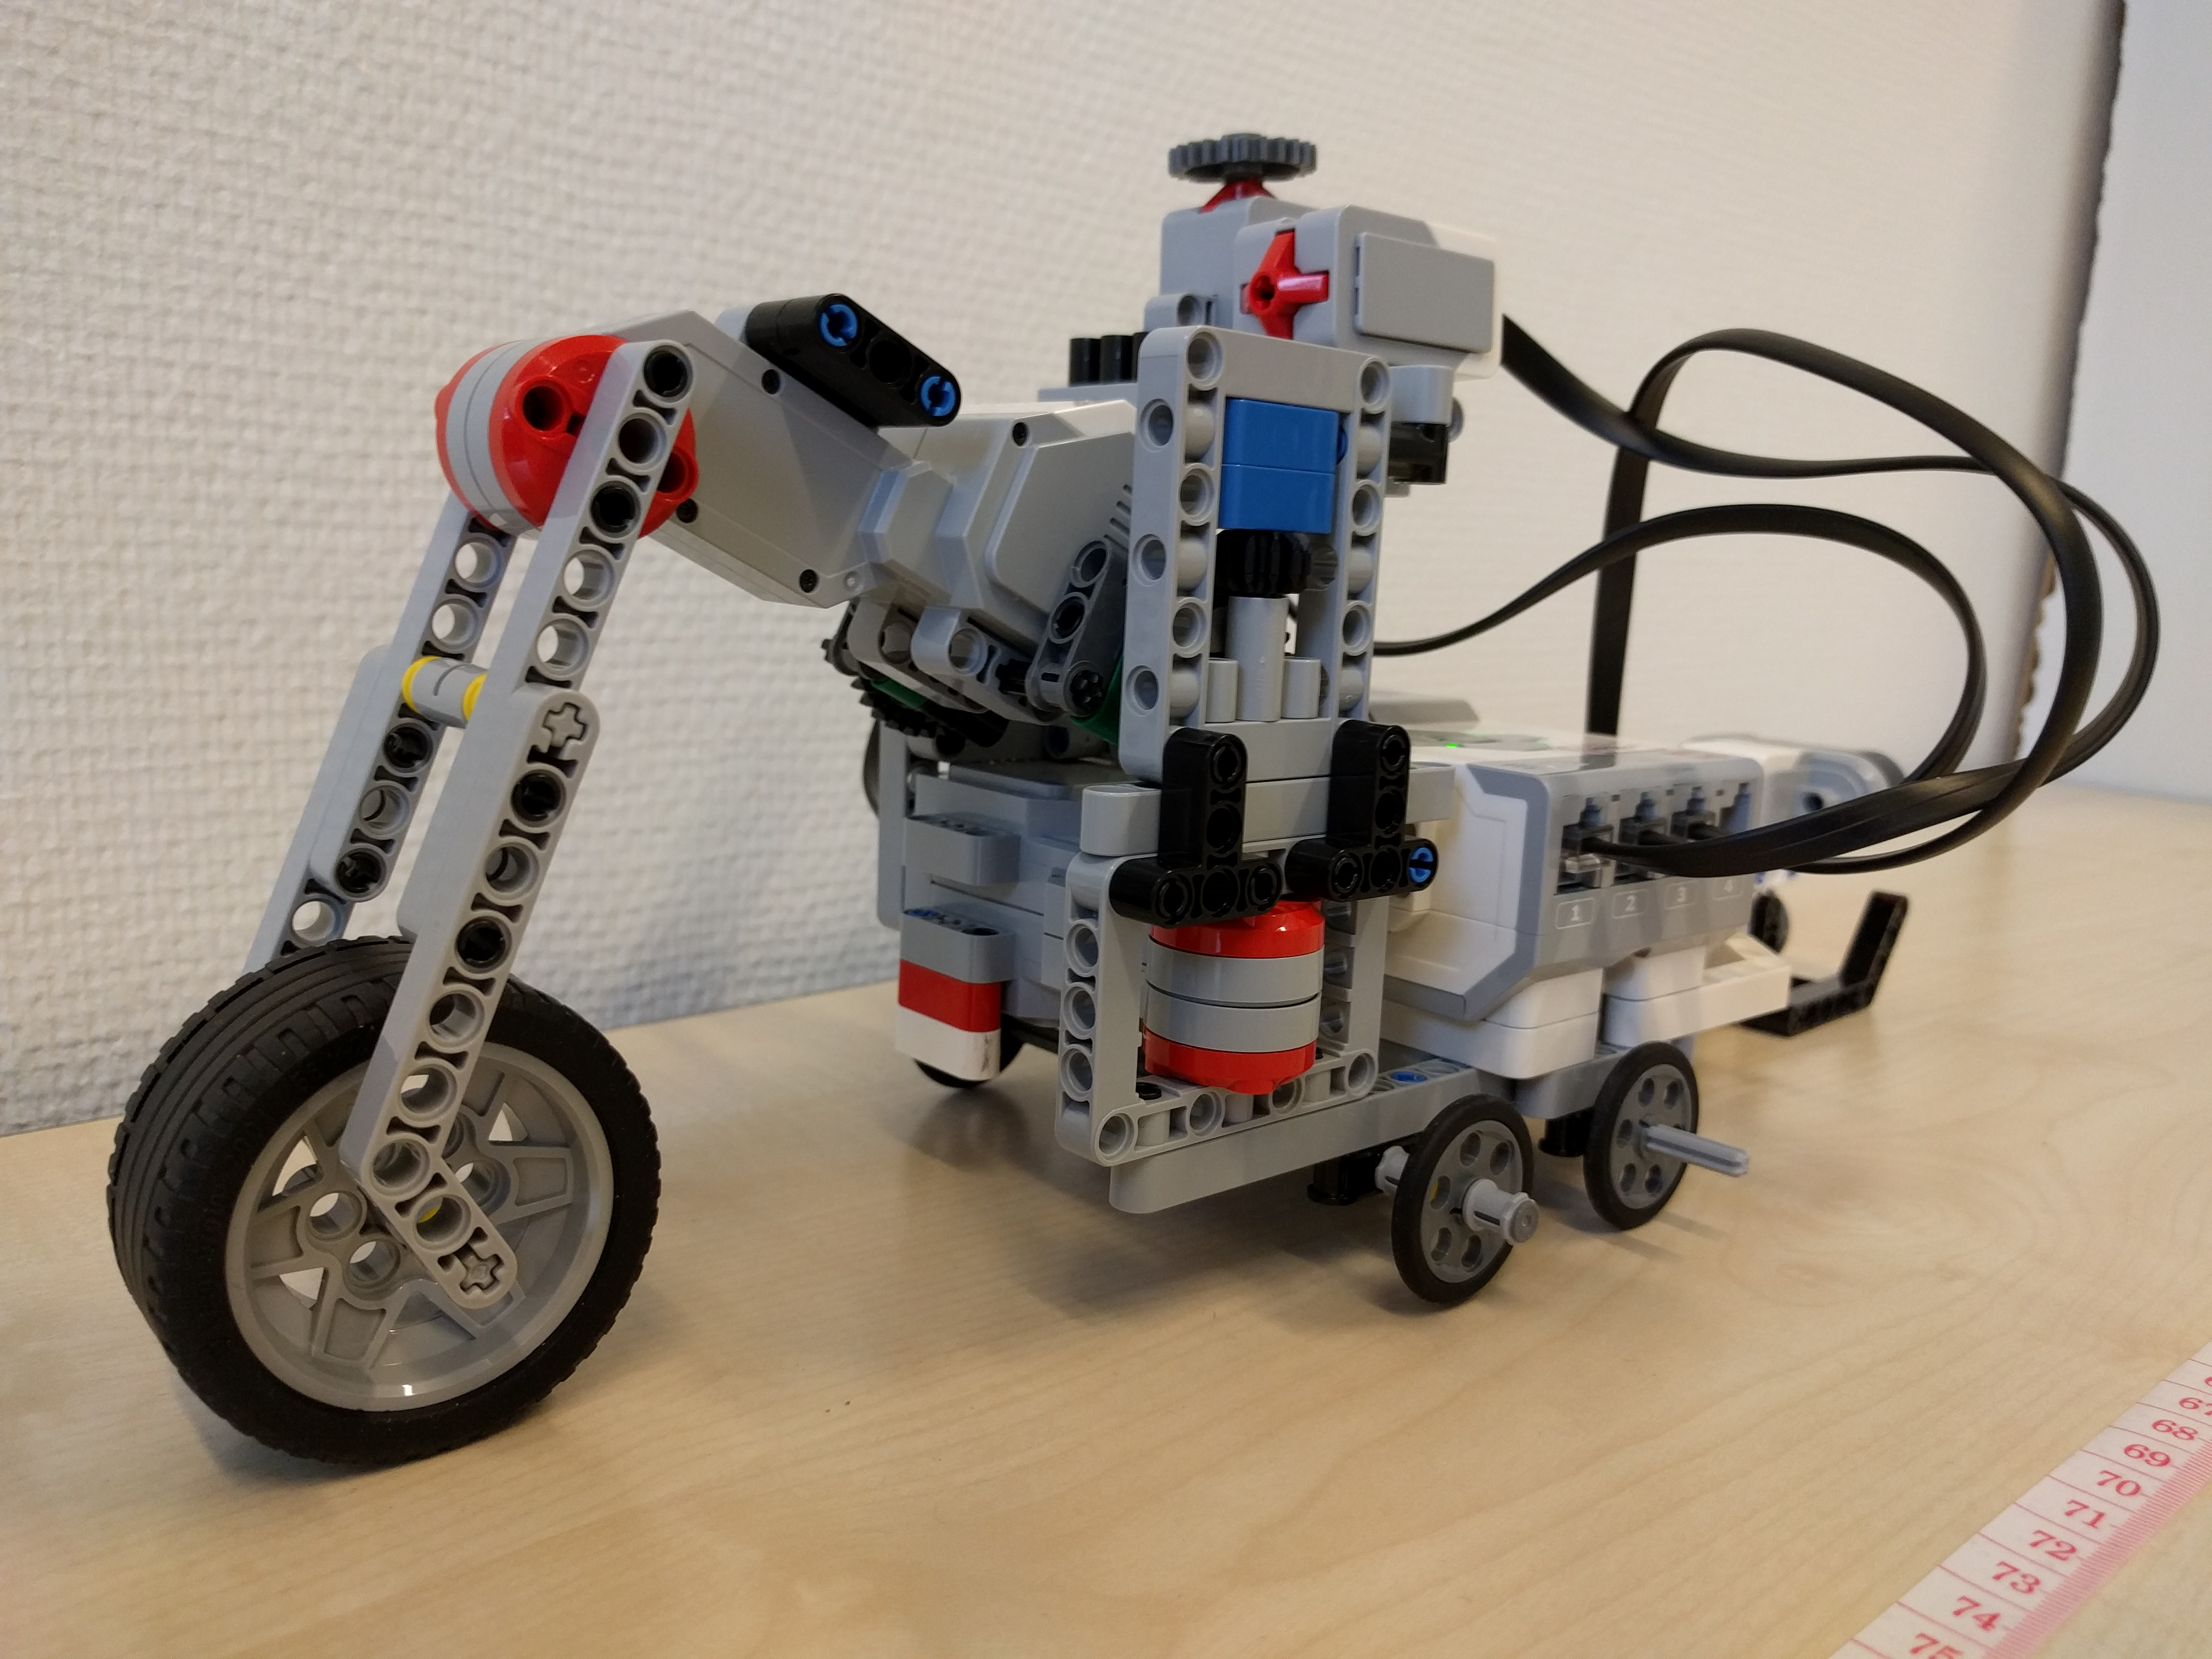
\includegraphics[width=0.6\linewidth]{images/crawl_robot}
	\caption{Crawl Robot, frontal view.}
	\label{fig:crawl_robot}
\end{figure}
To demonstrate reinforcement learning in educational settings, we seek to have a physical model for demonstration. The training process should be robust, as to deliver a reliable demonstration in teaching scenarios outside of laboratories, and fast, to keep the attention of an audience. While many robot designs and learning goals, like pole balancing or swinging, are possible, we selected a crawling robot as a suitable object for demonstration. The concept of a robot using one arm to crawl, or drag itself along a linear track has been explored by multiple other studies \cite{youtube_crawl2} \cite{youtube_crawl}. We selected this task, as it is a comparatively simple design, with few moving parts. The system is more robust towards external force from curious bystanders than for example a loosely swinging pole. By Defining a limited state space we can simplify the problem and get a training time suitable for demonstration. Realizing this robot will provide us with a model for demonstration  and equip us with the experience and knowledge to solve more complex problems in the future.


\subsection{Robot Design}
To facilitate the crawling motion, the robot needs a movable arm to pull itself forward. The arm consist of two elements: the base arm, which is attached to the robot, and a pivot arm attached to the base arm. Both arm joints rotate around the same axis, allowing the hand at the far end of the pivot to move on a plane. To allow the arm to pull the robot, the ground friction of the arm has to be maximized, and the ground friction of the robot minimized. This is achieved by a big rubber tyre firmly attached (not spinning) to the robots hand. The robot body sits on wheels which can spin freely. See Figure \ref{fig:crawl_robot} for a photo of the robot arm, hand and wheel basis.

To measure distance travelled, the ultrasonic sensor is used. This sensor is attached to the back of the robot and records the distance to a target from the rear end of the robot. As the wheel basis of the robot might tilt when the arm is pressing into the ground, while the ultrasonic sensor requires a stable angle towards the target for consistent measurements, the sensor is mounted on a sled which is pulled behind the robot. The sled is visible in figure \ref{fig:sub2}.

To calibrate the motors of the arm, two buttons are attached to the top of the robot. During the start up process, the arm is moved all the way back, until base arm and pivot arm hit their respective buttons. This motion is depicted in Figure \ref{fig:sub1}. The certainty about the arm position attained by this action is used to initialize the 0-angle of both motors.

\begin{figure}
	\centering

	\begin{subfigure}{.4\textwidth}
		\centering
		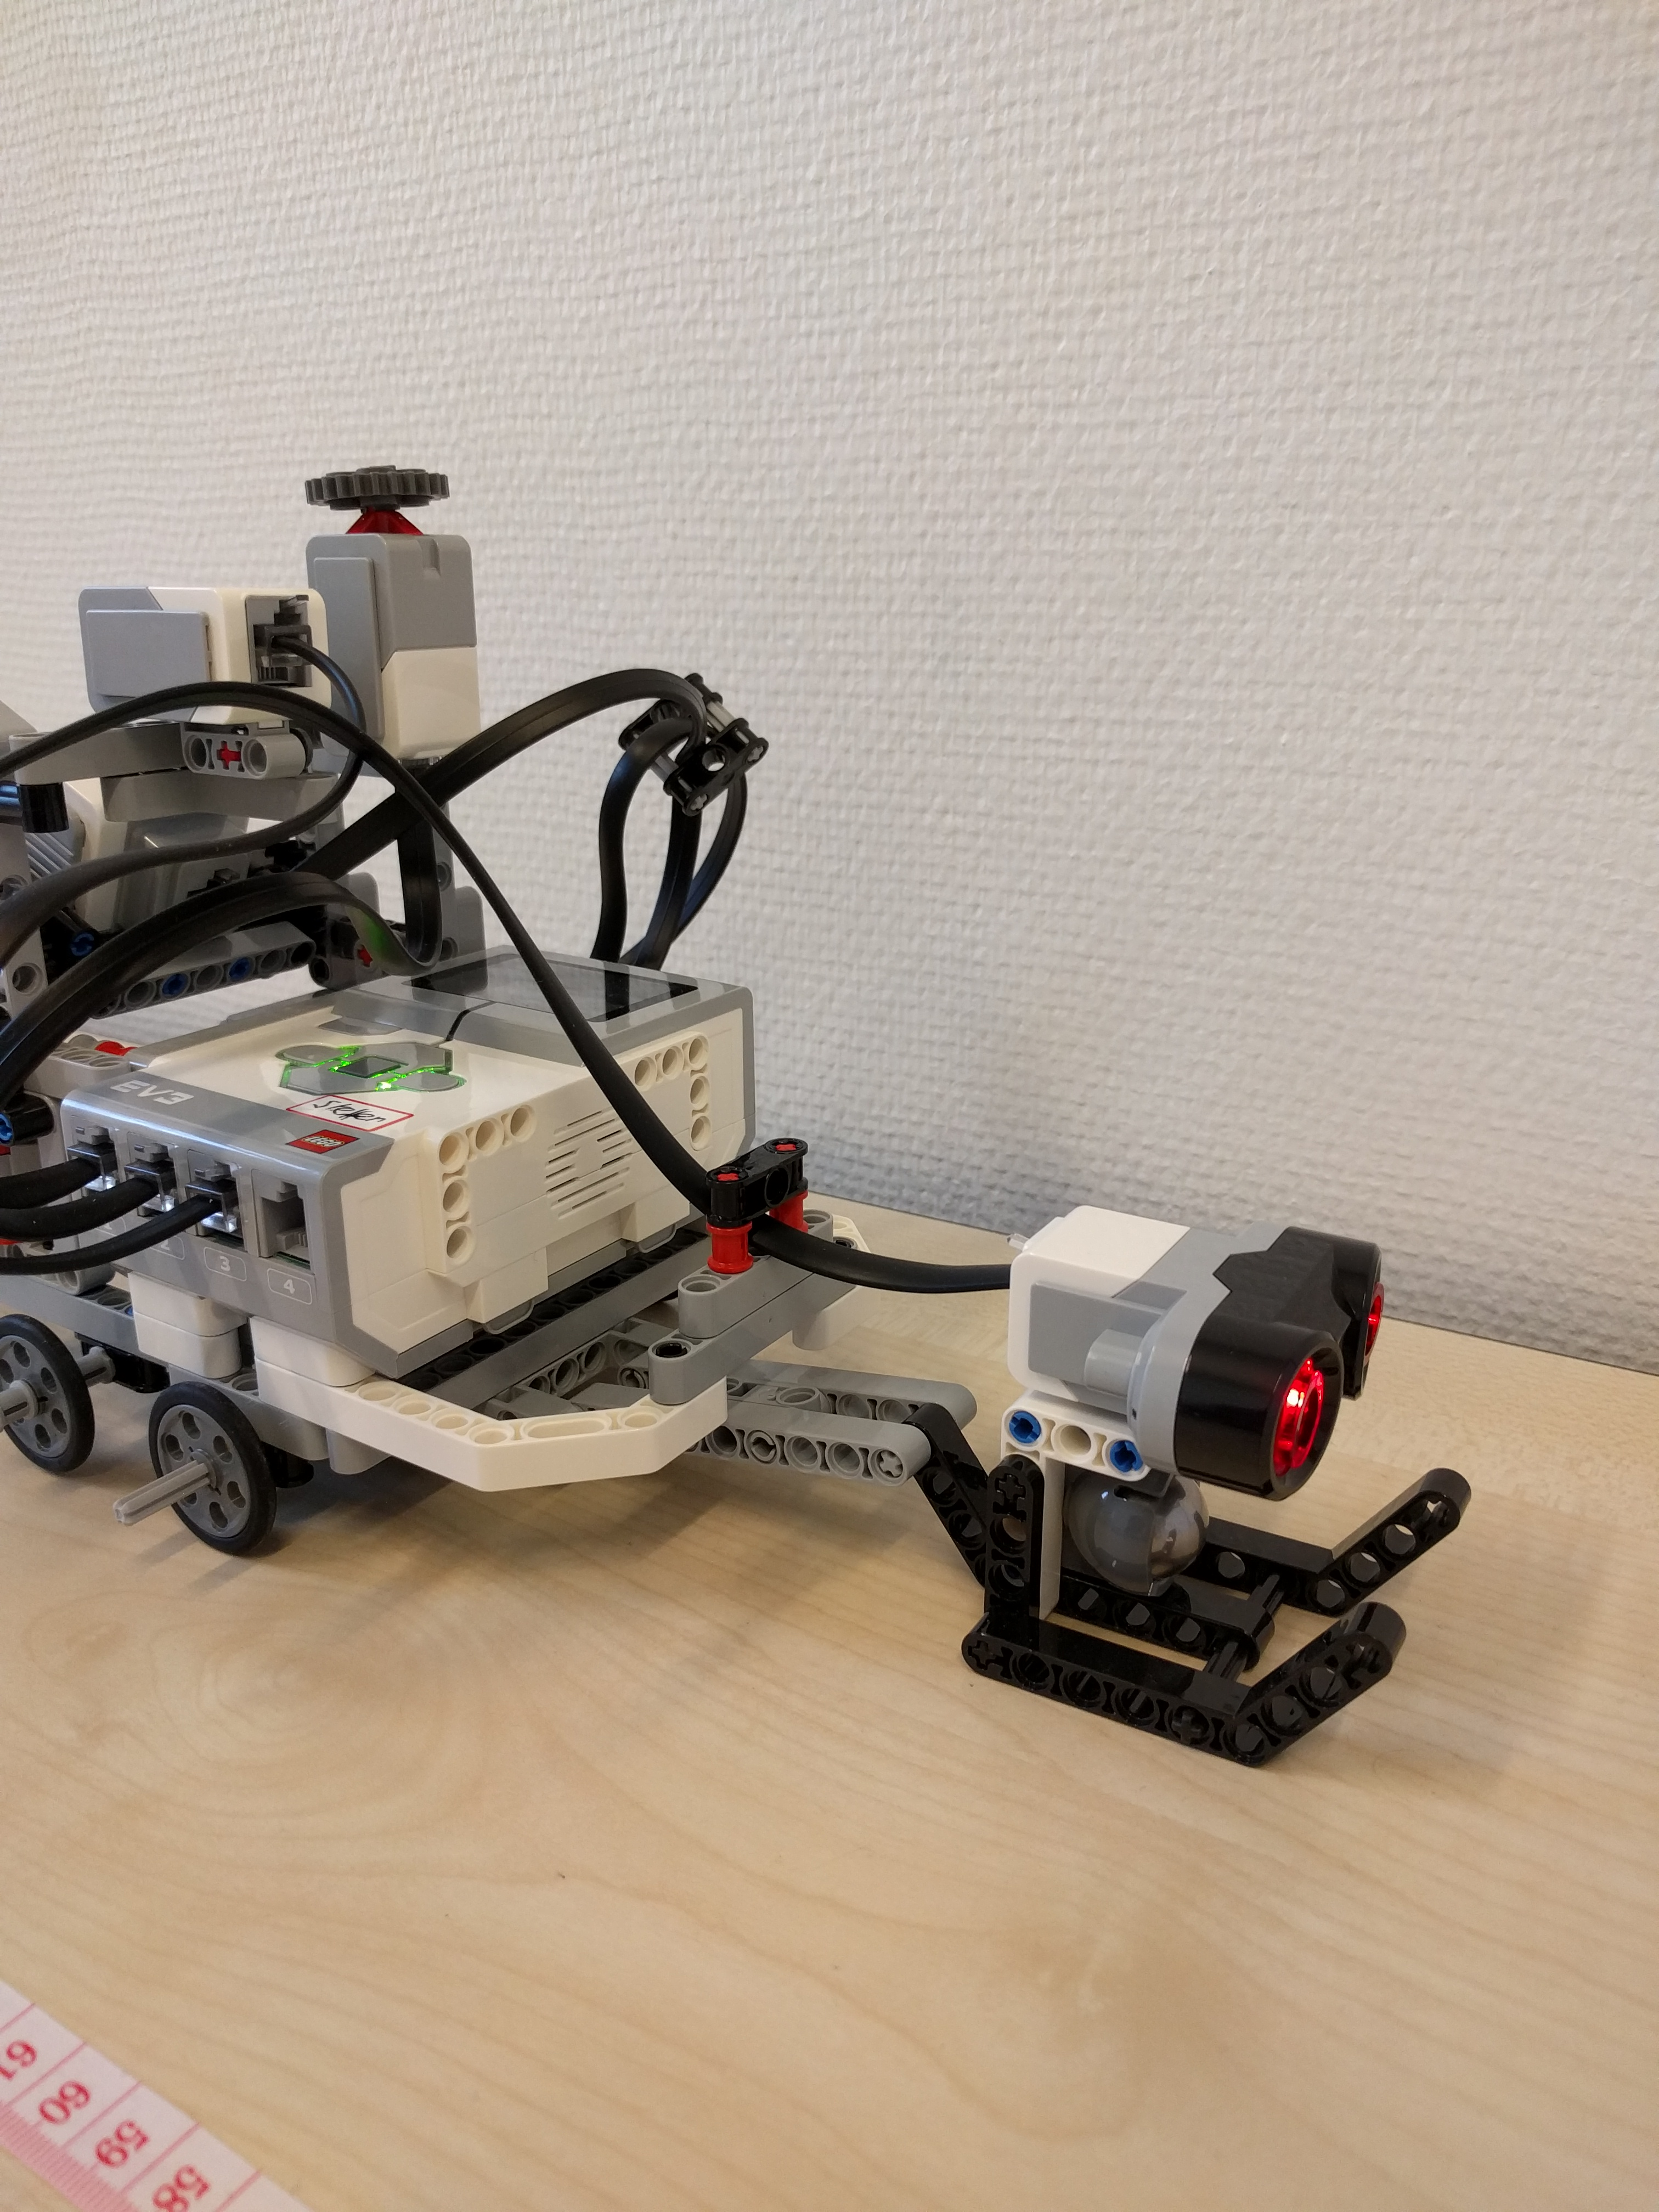
\includegraphics[width=0.8\linewidth]{images/crawl_sled}
		\caption{Ultrasonic sensor on a sled at the back of the robot.}
		\label{fig:sub2}
	\end{subfigure}
	\begin{subfigure}{.4\textwidth}
		\centering
		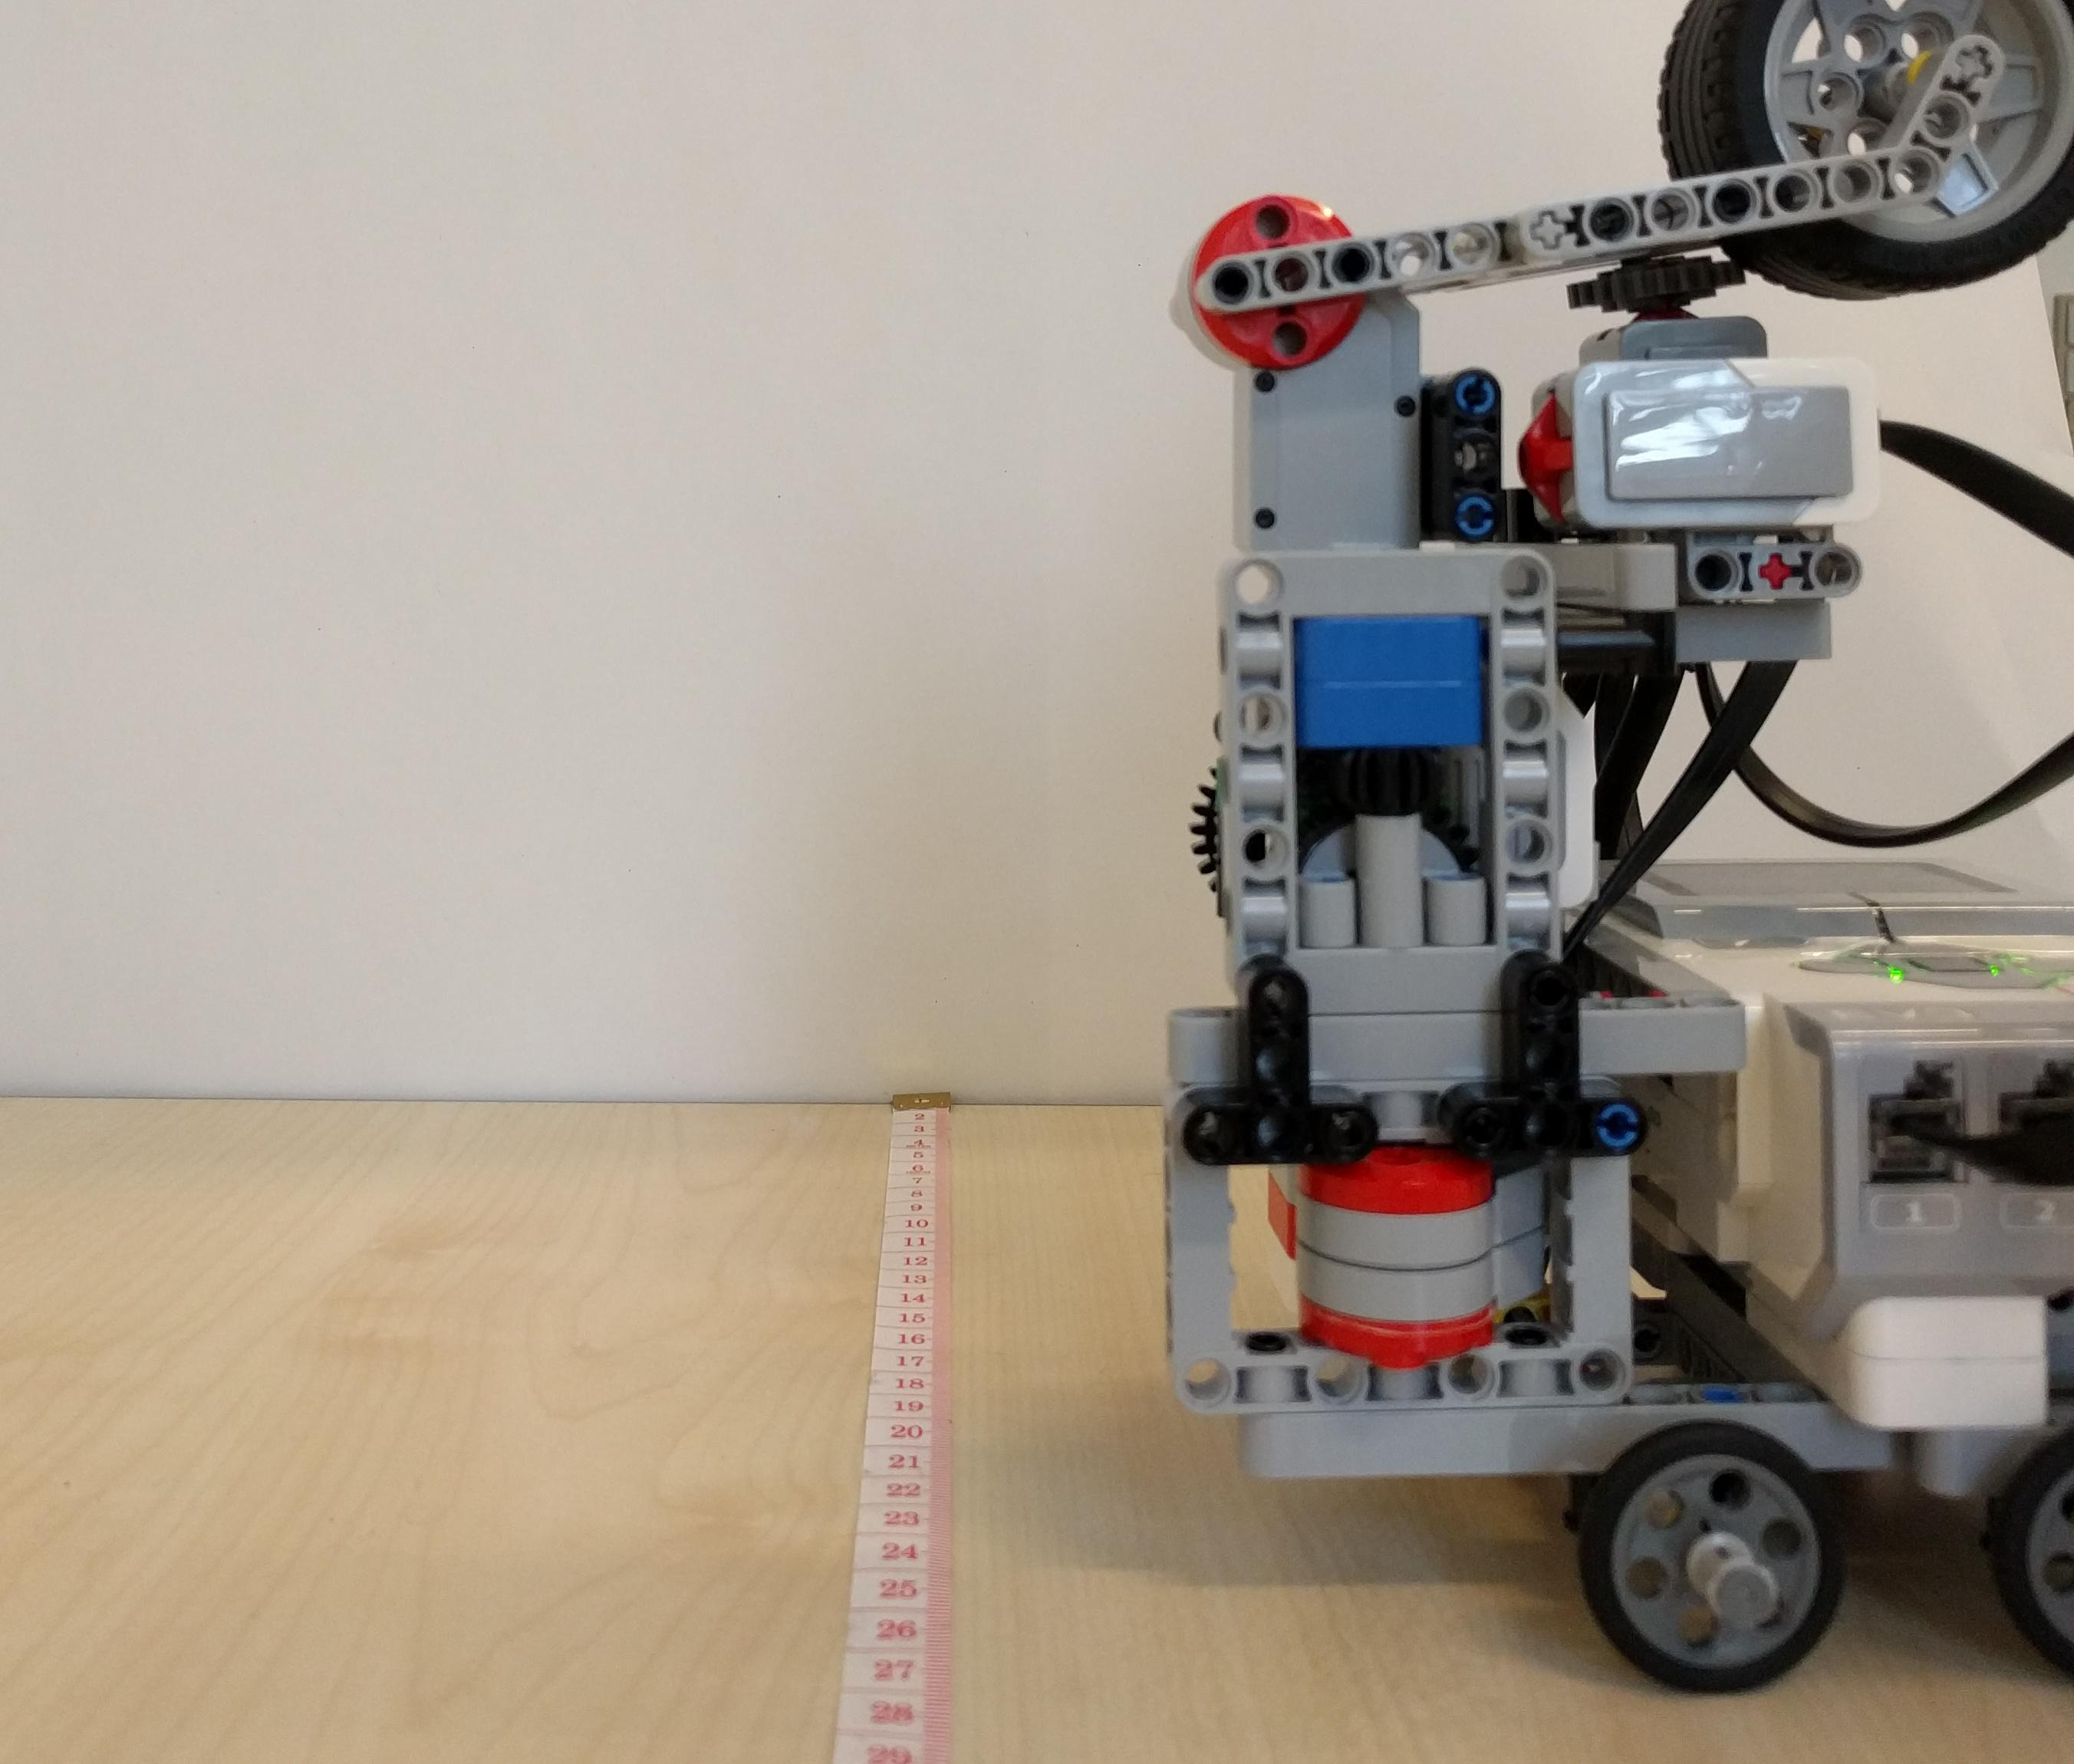
\includegraphics[width=1\linewidth]{images/crawl_calibrate}
		\caption{calibrating motion of the crawl robot.}
		\label{fig:sub1}
	\end{subfigure}%
	\caption{Designs of the Crawl Robot}
	\label{fig:test}
\end{figure}

\subsection{Formulation of the Learning Problem}
To train the robot how to crawl, we use Q-learning. Q-learning is a form of reinforcement learning. It provides agents with the capability of learning to act optimally in Markovian domains by experiencing the consequences of actions. To learn, an agent tries an action at a particular state, and evaluates its consequences in terms of the immediate reward or penalty it receives and its estimate of the value of the state to which it is taken. By trying all actions $A$ in all states $S$ repeatedly, it models the value $Q(s,a)$ of each action state pair. The algorithm learns which state-actions pairs are the best overall, judged by long-term discounted reward \cite{Watkins1992}.

\begin{figure}
	\centering
	\includegraphics[width=0.6\linewidth]{images/crawl_states}
	\caption{Arm positions (states) of the crawl robot. From top to bottom: Pivot arm in positions far, mid, close. From left to right: Base arm in positions up, mid, down. The tilt of the robot base in the right column is caused by the arm pressing into the floor.}
	\label{fig:crawl_states}
\end{figure}
\medskip
The Q-learning algorithm fits the domain of the crawl robot. The implementation chosen is shown in Algorithm \ref{alg:q-learn} and follows \cite{sutton1998introduction}. Training is grouped into epochs, and each epoch consists of multiple steps (loops in line 2 and 4 of the algorithm). In each step, we take one action. This action is determined with the $\epsilon$-greedy strategy (lines 5-10), where with probability $\epsilon$ we perform a random action, and with probability $1-\epsilon$ we greedily select the action $a$ with the highest current value. In line 11 we perform the sampled action $a$, observe the reward $r$ and transition into the next state $s'$. In line 12 the state value function $Q(s,a)$ is updated. We end the step by setting $s \leftarrow s'$ and then repeating (line 13, 14). Each epoch starts with start state $s_0$. To execute the learned policy, we set $\epsilon$ to $0$ and no longer update the state value function.
\medskip

To apply Q-learning to the crawl robot domain, we model an action as moving the arm. The immediate reward or penalty received is proportional to the distance traveled by performing the action, as measured by the ultrasonic sensor. As learning speed is of importance, we define a discrete state space with 9 states. These states are displayed in figure \ref{fig:crawl_states}. By selectiong the state space to be small, the learning algorithm has to explore only few states, which speeds uo learning. We could have sub divided the arm movement plane into more states, with the drawback of longer learning time. More formally, the choices for the action-space $A$ and state space $S$ are:
\begin{align*}
	A = \{ &\text{ move base arm up}, \text{ move base arm down} , \text{ move pivot arm far}, \text{ move pivot arm closer}\} \\
	S = \{ &\text{base up pivot far}, \text{ base mid pivot far}, \text{ base down pivot far}, \\
	       &\text{base up pivot mid}, \text{ base mid pivot mid}, \text{ base down pivot mid},\\
	       &\text{base up pivot down}, \text{ base mid pivot down}, \text{ base down pivot down},\} \\
\end{align*}
The initial state for each epoch is given by $s_0 = \text{base up pivot far}$, which is the furthest extension of the arm. For fast learning, we got good results with a learning rate $\alpha = 0.5$, discount rate $\gamma = 0.8$. The exploration factor $\epsilon$ is initially set to $0.5$ and declines exponentially throughout training, allowing lots of exploration at the start of training, while gradually reducing exploration for later epochs. We chose $35$ steps per epoch, as this amount allows each epoch to explore all states multiple times. Training is stopped once the motion appears to be executed with little error.

\begin{algorithm}[]
	\SetKwInOut{Input}{Input}
	\SetKwInOut{Output}{Output}
	
	\Input{learning rate $\alpha \in ]0,1]$, discount rate $\gamma \in [0,1[$}
	initialize $Q(s, a)$ with $0$ for all $s,a$\\
	\ForEach{epoch}
	{
		return to initial state $s_0$ \\
		\Repeat{epoch end}
		{
			sample $x$ uniform at random for $[0,1]$ \\
			\eIf{$x < \epsilon$}
			{sample $a$ at random}
			{select $a \leftarrow \arg \max_a(Q(s,a))$}	
			take action $a$, observe $r, s'$ \\
			$Q(s,a) \leftarrow Q(s,a) + \alpha [r + \gamma \  max_{a'} Q(s', a') - Q(s,a)]$ \\
			$s \leftarrow s'$
		}
		
	}
	\Output{state value function $Q$}
	\caption{Q-learning with $\epsilon$-greedy exploration}
	\label{alg:q-learn}
\end{algorithm}





\subsection{Results}
The crawl robot was trained using tabular Q-learning with the parameter choices stated in the previous section. In this section we discuss the training process and the learned result. For training, the robot is placed on a linear track. At the back of the robot, a solid target is placed to act as a point for range measurement by the ultrasonic sensor. During training, the robot explores actions and moves back and forth on the linear track. 

After 20 minutes of training, the learned motion appeared near perfect and training was stopped. This corresponds to 65 epochs of training, for a total of 2275 actions. The reward gathered in each epoch is plotted in figure \ref{fig:crawl_reward}. We can see that the reward gathered in each epoch has a clear upward trend, indicating that the robot got progressively better at the task. The exploration factor is exponentially declining, as shown in figure \ref{fig:crawl_exploration}. This leads to less exploration in later epochs. The result of this is visible in the reward plot, as in later epochs the results get more consistent.

The robot is not fully autonomous during training. It requires human intervention in three cases:
\begin{itemize}
	\item The ultrasonic sensor has a maximum range of 250cm. If the robot moves further away from its range measuring target, it can no longer track rewards. Similarly, if it pushes into the range finding target, it can not move further into the direction of the target. Both cases disrupt assessing the rewards of actions. To handle these cases, the robot will interrupt training when it gets too close to either end of the spectrum. Training is resumed once the robot is manually placed on a valid part of the training track.
	\item To properly assess the range to it's range measuring target, the ultrasonic sensor needs to be orthogonal to the target. If the robot rotates during training, the angle to the range finding target can change. An angle significantly different from 90 degrees leads to skewed reward tracking, and in special cases the sensor can no longer find the target, which prohibits range measuring entirely. If the orientation of the robot changes significantly, it has to be manually rotated to its initial position.
	\item In rare cases, the motors of the arm have slightly too little torque to push against resistance caused by the hand hitting the floor. The motors become stuck. In these cases the robot needs to be slightly pushed to overcome the resistance and release the motors.
\end{itemize}

A recording of the full training and a presentation of the learned motion is accessible as a video online at \cite{youtube_crawl_training}. The video shown the training process at 7 times normal speed. Manual interaction is shown as well.

\begin{figure}
	\centering
	\begin{subfigure}{.48\textwidth}
		\centering
		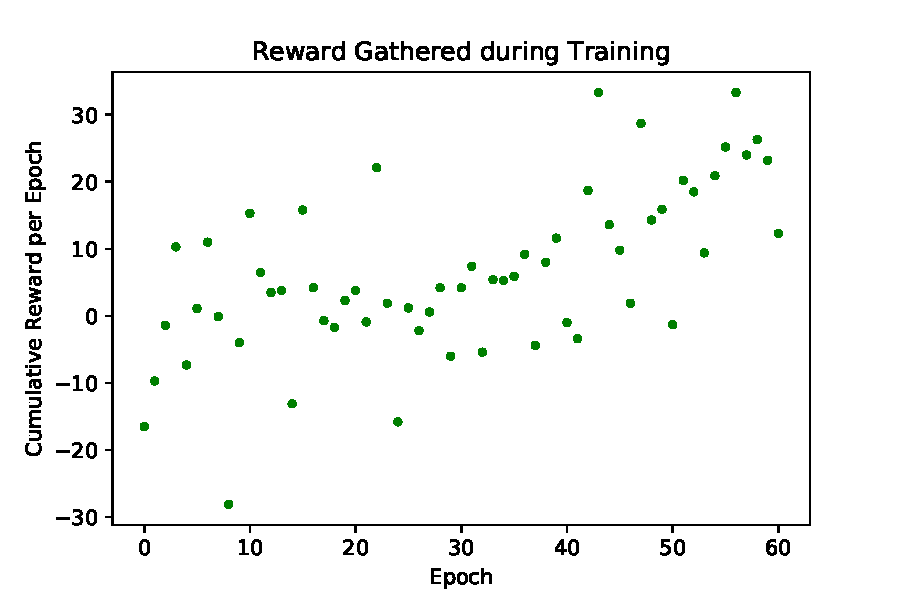
\includegraphics[width=1\linewidth]{images/crawl_rewards}
		\caption{Reward gathered per Epoch. An improvement is clearly visible.}
		\label{fig:crawl_reward}
	\end{subfigure}
	\begin{subfigure}{.48\textwidth}
		\centering
		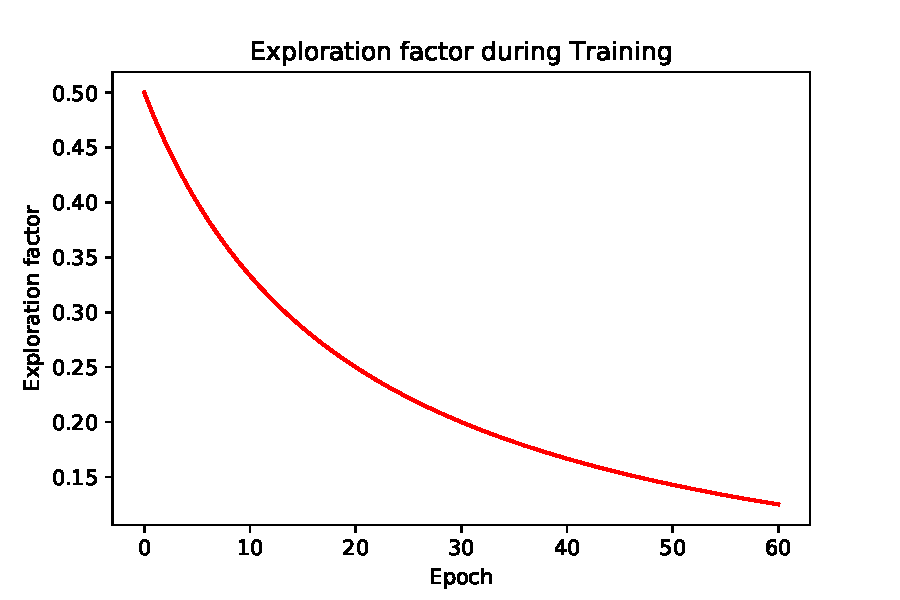
\includegraphics[width=1\linewidth]{images/crawl_exploration}
		\caption{Exponential decline of the exploration rate.}
		\label{fig:crawl_exploration}
	\end{subfigure}%
	\caption{Q-learning of the Crawl Robot}
	\label{fig:crawl_train}
\end{figure}


\subsection{Discussion}
With the presented framework, the crawling robot is able to learn a forward crawling motion in 20 minutes. As the training process requires constant human interaction for resetting the robot, we think this amount training time is appropriate. Especially in educational settings it should be considered as an upper limit. Since the training is interactive, observing how the robot develops an increasingly stronger forwards drive during training is quite rewarding to the observer. 

The learned motion is not smooth and appears abrupt, which results from the use of a discrete state space. Learning a crawling motion with this robot on a continuous state space has the potential of leading to a smoother, and possibly faster movement. A possible drawback is increased training time. Moving the arm on a continuous state space is a topic for future research.

The robot construction can be improved in the future. The current design has some mechanical issues, such as the strength of the motors in the arm and a tendency to slightly drift off the linear direction of movement. These problems could be addressed by re-constructing the robot and track of movement. A guide rail could constrict sideways the movement and gear conversions in the arm can be used to increase torque. The need for human supervision could be reduced by introducing a third motor to automatically move the robot back to its starting position after every epoch.

\medskip
In conclusion, we build a one-armed robot using LEGO parts, motors and sensors. We formulated a tabular q-learning problem with the goal of teaching the robot how to crawl. With some human interaction, the robot learned a forward crawling motion in 20 minutes. 




\pagebreak
\section{Swing-Robot}
\subsection{Problem}
The swing was made as a more complicated reinforcement learning task, inspired by a similar robot found on youtube\cite{youtube_swing}. In this setup, the robot has to learn to swing, in our case, by swinging one or both legs back and forth, and will receive higher rewards the higher it swings. This creates several layers of complexity. The task itself is non-trivial, and tabular learning as we used for the crawling robot may be insufficient, but we're also working against gravity, and need to be able to update and react often enough. Finally, there is a case for making this problem recurrent, introducing another layer of complexity.
\subsection{The Robot}
The two basic robot designs seen in the video that inspired this idea\cite{youtube_swing} can be described as a "crouch"-style swing, in which the robot does up-down body movements, and a "pull-up"-style swing, in which the robot moves legs/limbs to swing.

We decided to go for a "pull-up" style swing, with two legs that can move independently. See Figure \ref{fig:swing_robot}.

\begin{figure}[H]
	\centering
	\begin{subfigure}{.48\textwidth}
		\centering
		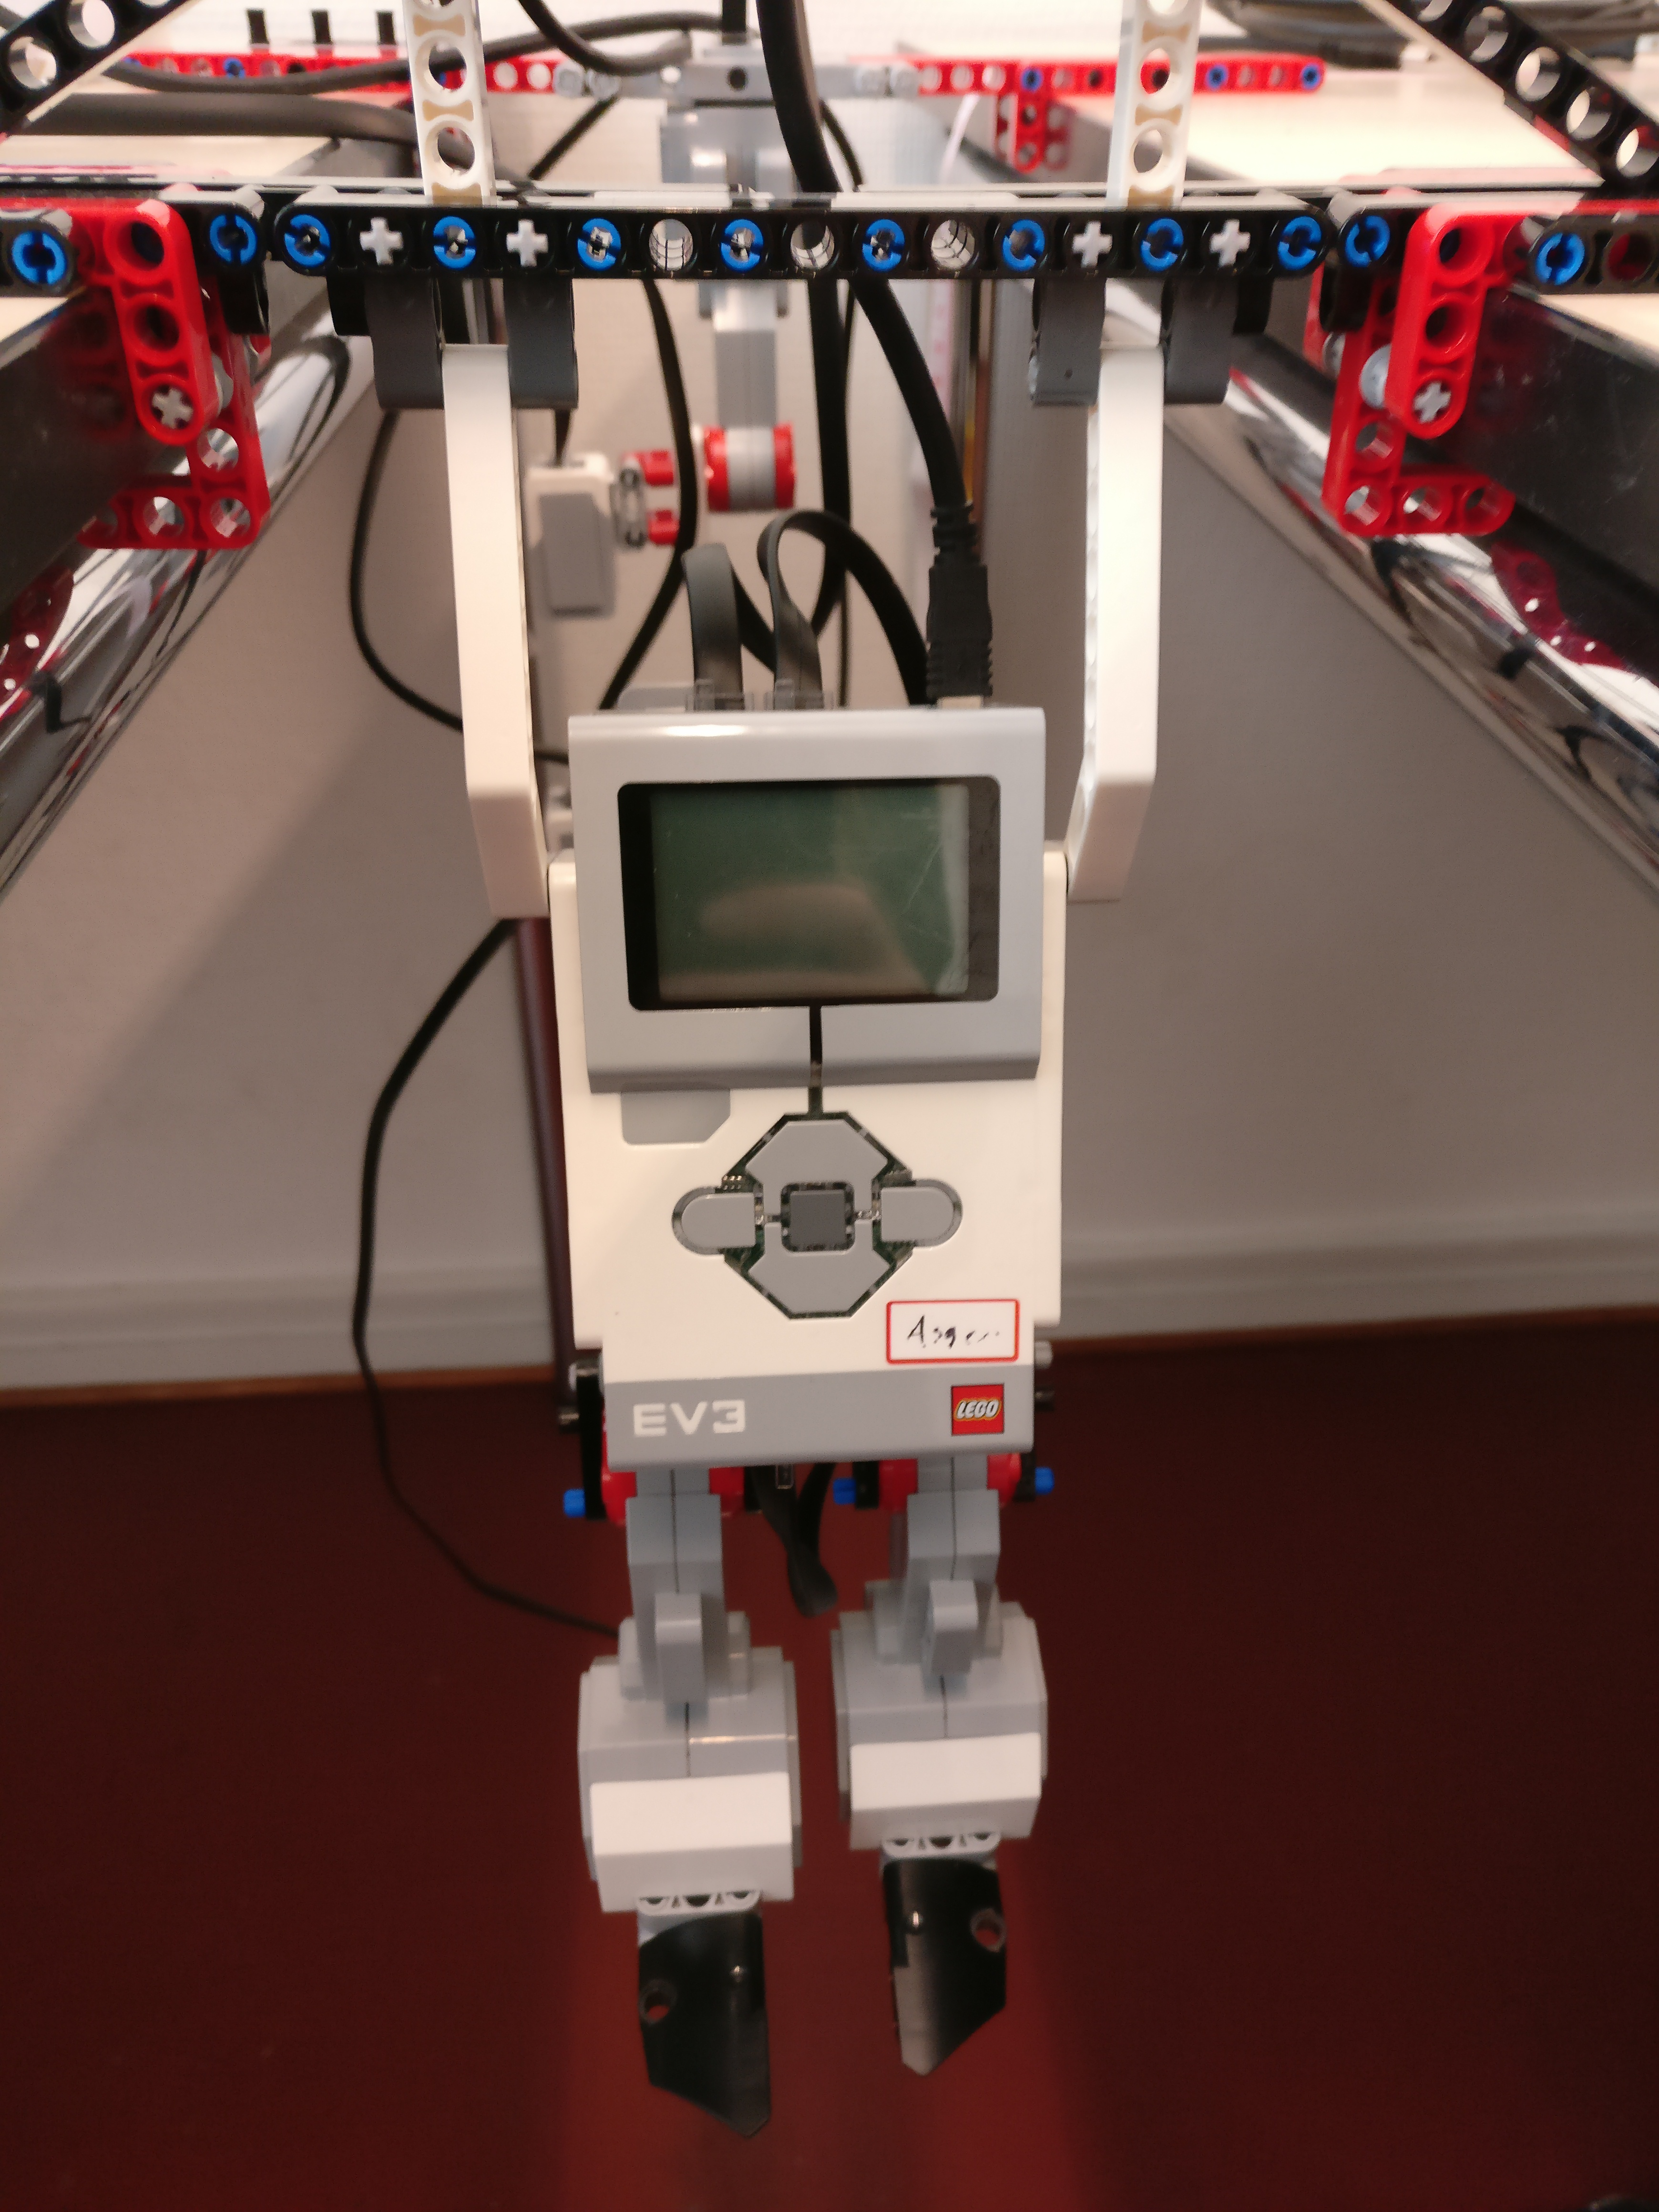
\includegraphics[width=1\linewidth]{images/swing_robot_front}
		\caption{Swing robot seen from the front. At the top of the picture you can see the robot mount lodged between two tables.}
		\label{fig:swing_robot_front}
	\end{subfigure}
	\begin{subfigure}{.48\textwidth}
		\centering
		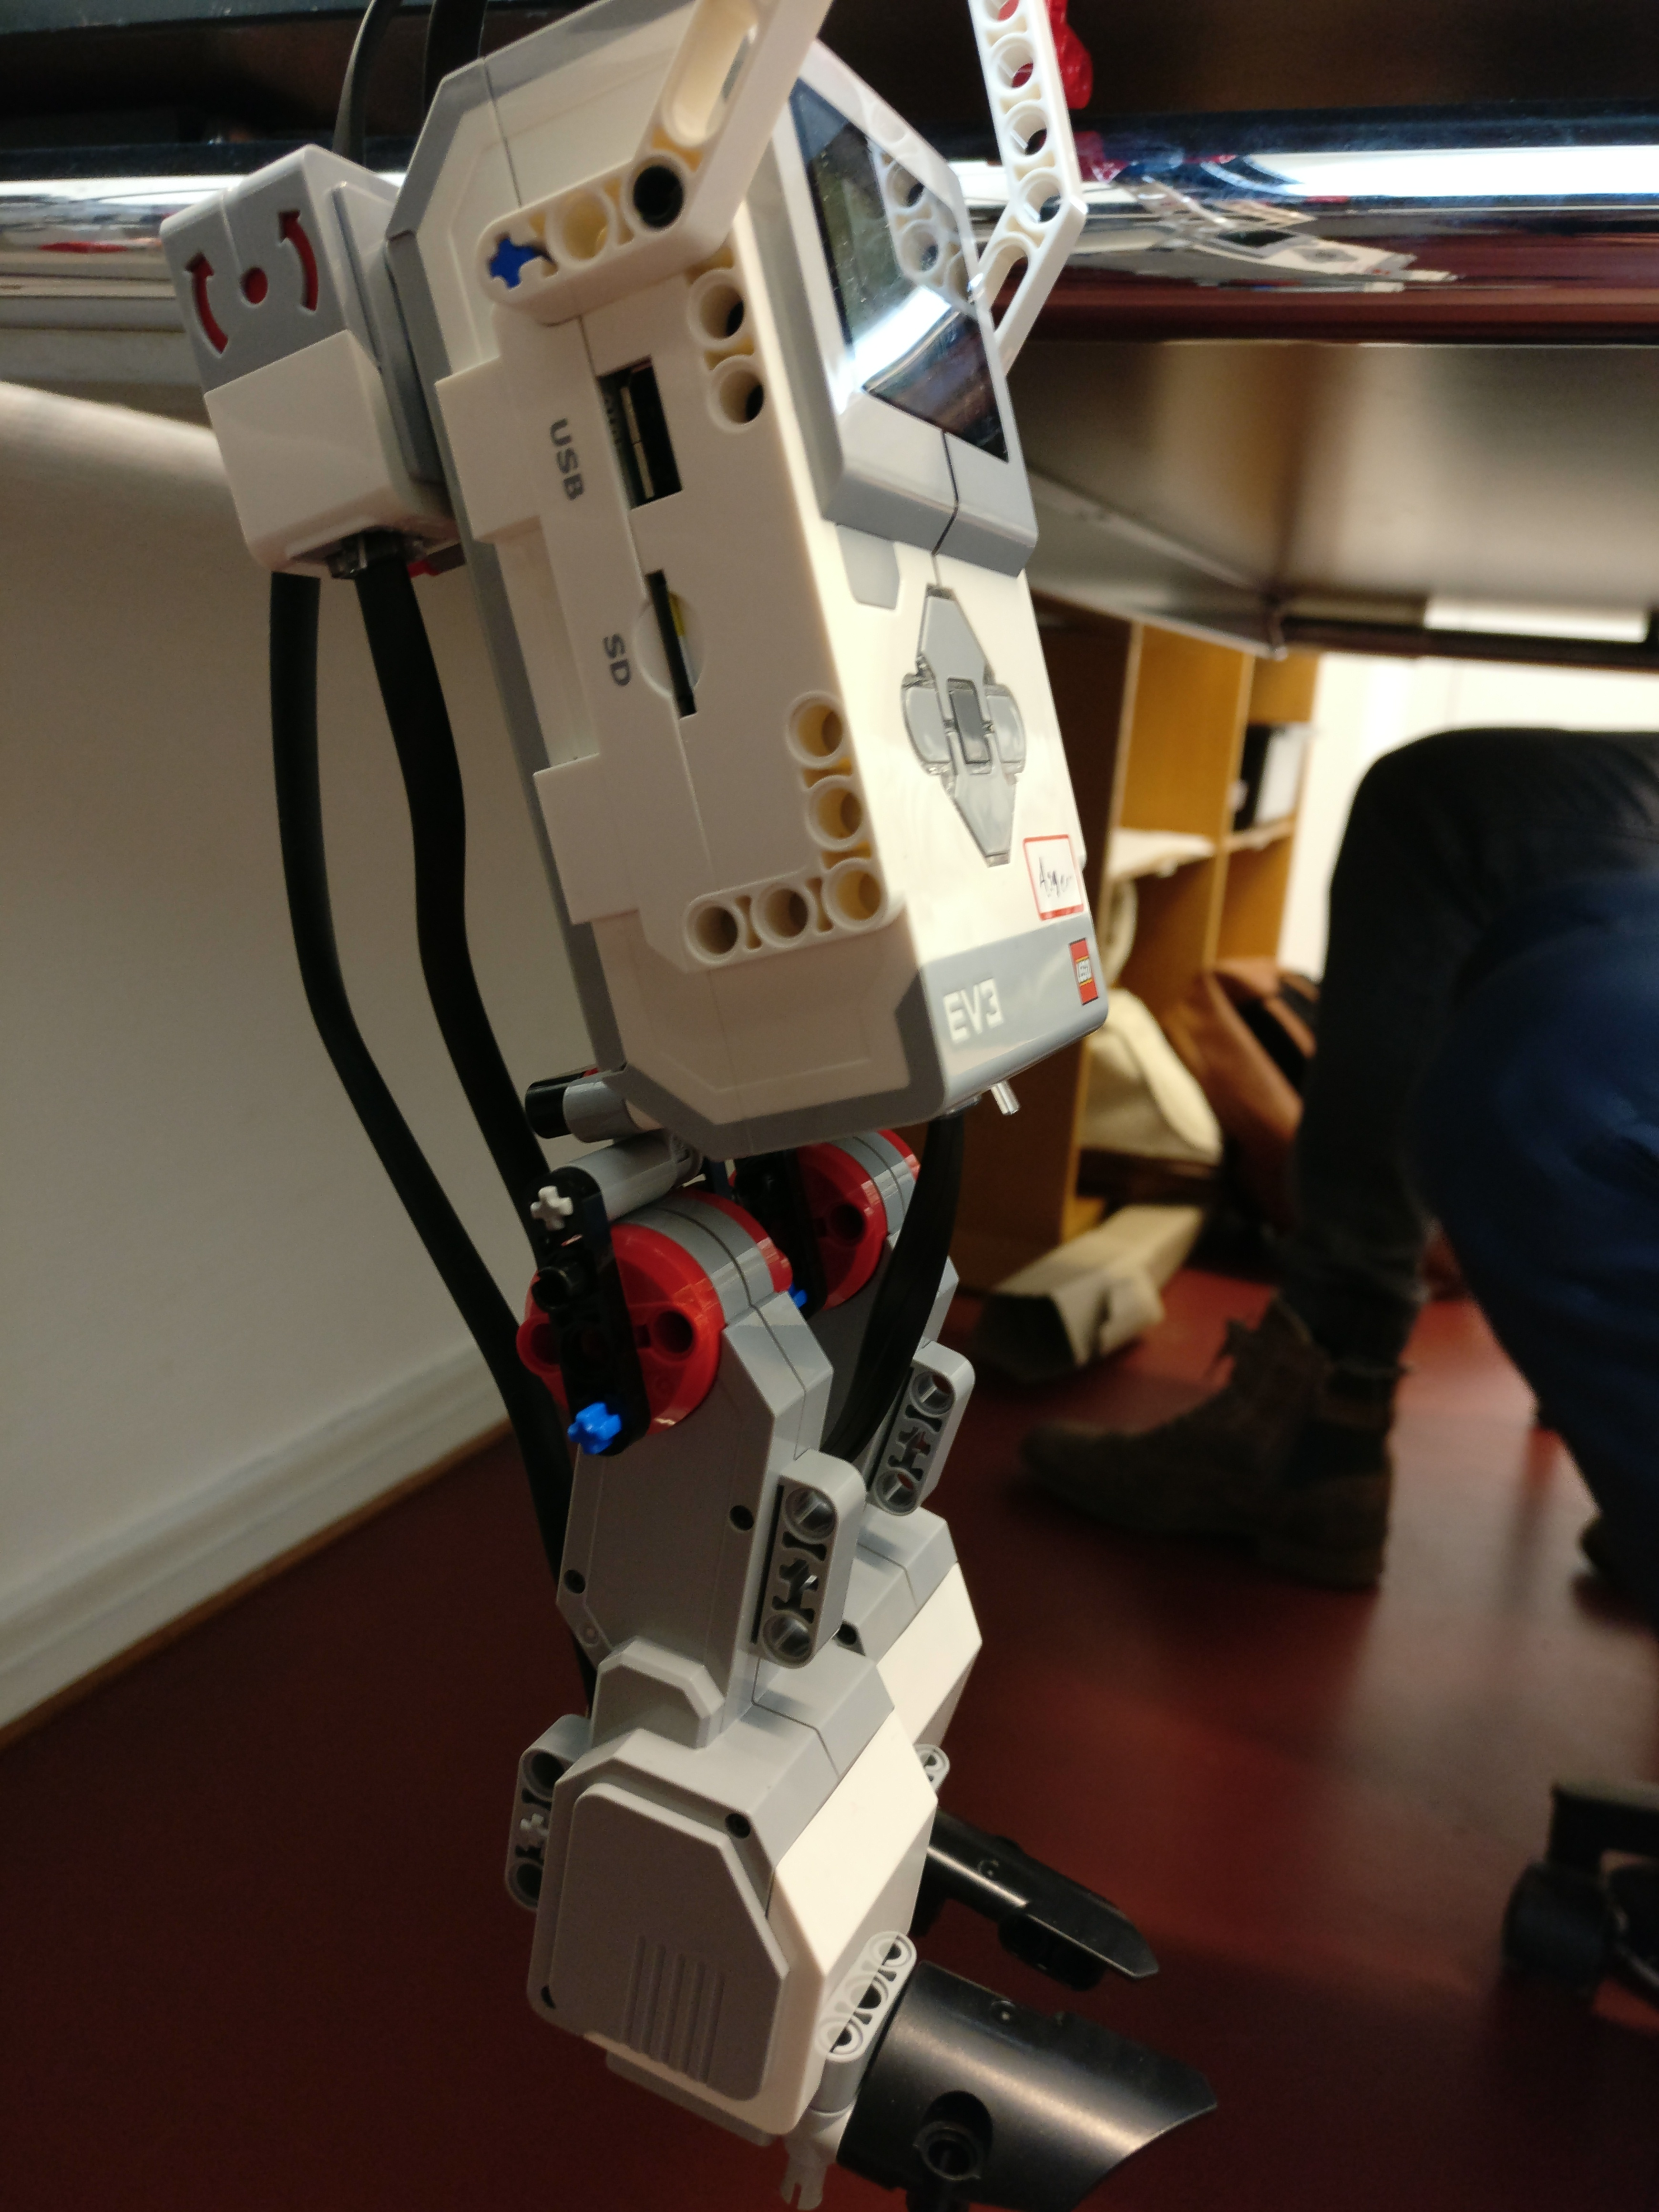
\includegraphics[width=1\linewidth]{images/swing_robot_side}
		\caption{Swing robot seen from the side, here the gyroscope and the leg mounting is visible.}
		\label{fig:swing_robot_side}
	\end{subfigure}%
	\caption{The Swing robot design. The legs can move independently, while the 'arms' swing freely on a bar. A gyroscope is mounted on the back of the robot.}
	\label{fig:swing_robot}
\end{figure}

To be able to swing, the robot must move some amount of counterweight, this is achieved by having each "leg" consist of a large motor mounted backwards, such that the motor part is moved, see Figure \ref{fig:swing_robot_side}.
On the back of the robot, a gyroscope is mounted, to measure angle and acceleration. The height of the gyroscope was chosen to provide the most stable observations and the least drift in angle over time.

This design was chosen to allow for both easy and complicated setups, where the legs can be controlled together or individually.

Instead of creating a large swing frame, a mount was made to fit in between two tables, this proved to be very stable. An alternative with similar stability would be an aluminium (or equivalent) frame, which is available for future projects. This frame is visible in Figure \ref{fig:swing_robot_front}



\subsection{The Learning}
To train the swing robot, we implemented covariance matrix adaptation evolution strategy (CMA-ES). CMA-ES is regarded as the state of the art in evolutionary and numerical optimization, and we have adapted it for reinforcement learning. Evolutionary strategies optimize by creating new candidate solutions that can be seen as offspring of the previous candidate solutions, featuring a combination of qualities, maybe with some mutations.

For training the swing, an epoch consists of 30 seconds, and the reward was set to be the highest absolute acceleration achieved in the epoch.
\subsection{Results}
final results
\subsection{Discussion}
includes issues / future work
ability to move legs independently, better single-leg movement (when legs count as one), recurrent version, better response speed for more (better) sensor observations and faster motor controls
vibrations from size of swing
\section{Future Work}
Shared/independent
future robots/  multi actor learning
generalized systems (one system that can learn both crawling, swinging etc)


\section{Individual contributions}
Table \ref{tab:contributions} shows the individual contributions to the report by each of the graded students.
\begin{table}[H]
	\centering
	\begin{tabular}{l|l}
		Steffen & Asger \\ \hline
		Development Setup & Introductions\\
		Motor Accuracy & Time delays\\
		Ultrasound Sensor & Colour Sensor\\
		Calibration & Colour Detection\\
        Crawl Robot & Colour Robot \\
	     & Swing Robot: problem\\
	     & Swing Robot: robot design \\
	     & \\
     
		      
	\end{tabular}
	\caption{Sections of the report written by each of the students}
	\label{tab:contributions}
\end{table}


\bibliographystyle{abbrv}
\bibliography{references}

\end{document}
